\documentclass[12pt,fleqn]{article}


\usepackage[utf8]{inputenc}
\usepackage[T2A]{fontenc}
\usepackage{amssymb,amsmath,mathrsfs,amsthm}
\usepackage{mathtext}
\usepackage[russian]{babel}
\usepackage{graphicx}
\usepackage{lipsum}
\usepackage[footnotesize]{caption2}
\usepackage{indentfirst}
\usepackage{comment}
\usepackage{cmap}
\usepackage{hyperref}
\usepackage[export]{adjustbox}
%\usepackage[ruled,section]{algorithm}
%\usepackage[noend]{algorithmic}
%\usepackage[all]{xy}

% Параметры страницы
\textheight=24cm
\textwidth=16cm
\oddsidemargin=5mm
\evensidemargin=-5mm
\marginparwidth=36pt
\topmargin=-2cm
\footnotesep=3ex
%\flushbottom
\raggedbottom
\tolerance 3000
% подавить эффект "висячих стpок"
\clubpenalty=10000
\widowpenalty=10000
\renewcommand{\baselinestretch}{1.1}
\renewcommand{\baselinestretch}{1.5} %для печати с большим интервалом
% переименовываем  список литературы в "список используемой литературы"
\addto\captionsrussian{\def\refname{Список используемой литературы}}

\renewcommand{\baselinestretch}{1.1}
\renewcommand{\baselinestretch}{1.5} %для печати с большим интервалом
\DeclareMathOperator*{\argmax}{arg\,max}
\DeclareMathOperator*{\argmin}{arg\,min}
\DeclareMathOperator*{\E}{\mathbb{E}}
\DeclareMathOperator*{\cov}{\mathrm{cov}}
\DeclareMathOperator*{\Bs}{boldsymbol}

\newtheorem{definition}{Опр.}
% Дополнительные команды для личных обозначений
\pagestyle{plain}
\begin{document}

\begin{titlepage}
\begin{center}
    
	Московский государственный университет имени М. В. Ломоносова
	
    
\includegraphics[width=50mm]{msu.eps}

    \bigskip
    
    
    Факультет Вычислительной Математики и Кибернетики\\
    Кафедра Математических Методов Прогнозирования\\[20mm]

    \textsf{\large\bfseries
        КУРСОВАЯ РАБОТА \\[10mm]
        Обзор методов оптимизации гиперпараметров \\
        Review on hyperparameter optimization methods 
    }\\[15mm]

    \begin{flushright}
        \parbox{0.5\textwidth}{
            \textbf{Выполнил:}\\
            студент 3 курса 317 группы\\
            \emph{Швец Павел Игоревич}\\[5mm]
            \textbf{Научный руководитель:}\\
            д.ф-м.н., профессор\\
            \emph{Дьяконов Александр Геннадьевич}
        }
    \end{flushright}

    \vspace{\fill}
    Москва, 2020
\end{center}
\end{titlepage}

\newpage
\renewcommand{\contentsname}{Содержание}
\tableofcontents

\newpage
\begin{abstract}
    В данной работе производится обзор существующих методов оптимизации гиперпараметров. Рассматриваются подходы, использующие переборные стратегии и стратегии, использующие байесовскую оптимизацию. В работе проведены сравнительные характеристики в зависимости от выбора вспомогательной функции и структуры вероятностной модели использующиеся при байесовской оптимизации.
\end{abstract}

\newpage
\section{Введение}

    Существует множество различных моделей используемых в машинном обучении. Однако почти все являются парметризуемыми (такие параметры называют гиперпараметрами), настройку которых предлагается осуществлять пользователю. На этот процесс уходит достаточно много времени.
    Поэтому возникает потребность в быстрых и эффективных методах их настройки.
    
    
    Привычные градиентные методы оптимизации мало применимы в данной области, поскольку не всегда существует прямая функциональная зависимость между функцией качества (потерь) и гиперпараметрами.
    Далее приведён обзор существующих методов оптимизации гиперпараметров моделей. Приведены сравнительные эксперименты. 
    
    
    
\section{Постановка задачи}

Пусть дано некоторое семейство $\mathcal{A}$ алгоритмов, параметризуемое $N$ гиперпараметрами. Тогда будем обозначать $\Lambda_k$ -- пространство рассматриваемых параметров задаваемых для $k$-го гиперпараметра. Тогда общее пространство гиперпараметров алгоритма будем обозначать $\Lambda = \Lambda_1 \times \Lambda_2 \times \dots \times \Lambda_N$. Будем обозначать $\mathcal{A}_\lambda$ алгоритм, параметризованный вектором гиперпараметров $\lambda \in \Lambda$. 

Каждое из пространств $\Lambda_k$ может быть действительным (например, параметры EM-алгоритма для смеси нормальных распределений или темп обучения для стохастического градиентного спуска), дискретным (например, число соседей в методе K~--~ближайших соседей), бинарным (например, использование или нет early stopping при обучении нейронной сети). Обычно подразумевается, что пространство ограничено (в случае задания с помощью множества конечно). 

Также возможны ситуации, когда некоторые гиперпараметры не влияют на модель при не изменении других (например, если в модели параметризуется расстояние Минковского $p$, а рассматривается косинусное расстояние в методе K--ближайших соседей). 

\newpage

Пусть дана некоторая выборка $\mathcal{X}$, пусть также задана некоторый функционал качества $\mathcal{L}$. Тогда задачей является найти глобальный минимум следующего выражения:
$$\lambda_{*} = \argmin_{\lambda \in \Lambda} \underset{(\mathcal{X}_{train},\, \mathcal{X}_{valid}) \sim \mathcal{X}}{\E} V(\mathcal{L},\, \mathcal{A}_{\lambda},\, \mathcal{X}_{train},\, \mathcal{X}_{valid})$$

Здесь $\mathcal{X}_{train}, \mathcal{X}_{valid}$ -- некоторое разделение выборки для обучения и валдиации. Под $V(\cdot,\, \cdot,\, \cdot,\, \cdot)$ подразумевается функционал в виде функции потерь, который показывает качетсво алгоритма $\mathcal{A}_{\lambda}$, обученного на $\mathcal{X}_{train}$ и проверяющийся на $\mathcal{X}_{valid}$.

Поскольку рассматриваются выборки конечного размера математическое ожидание приближается с помощью различных стратегий валидации (например, Hold-out,\\ K-Fold, LOO, и т.д.), от выбора которой зависит затрачиваемое на подсчёт время.

Также иногда вводится параметр бюджета $T$, задающий ограничение на работу метода поиска параметра $\lambda_{*}$, примером тому может служить: максимальное количество итераций, максимальное время работы и т.д.

\section{Обзор существующих методов}
Ниже будут рассмотрены некоторые общие подходы и их модификации к решению поставленной задачи оптимизации гиперпараметров.

\subsection{Grid Search}
Один из самых используемых и простых методов при оптимизации гипрепараметров. Идея его заключается в переборе сетки задаваемых значений. Обычно данный метод используют при наличии соответствующих вычислительных ресурсов, поскольку его основным преимуществом является параллелизуемость. Ещё одним из преимуществ является применимость на всех структурных пространствах $\Lambda$. Поскольку сетка может содержать достаточно много узлов имеет место проклятие размерности. Пусть задано рассматриваемое структурное пространство $\Lambda$ (в случае Grid~Search оно дискретно), тогда число запусков обучения будет пропорционально зависеть от $|\Lambda| = \prod_{k=1}^{n}|\Lambda_k|$. Поэтому одновременно лучше настраивать небольшое количество параметров.
\subsection{Random Serach}
При использовании данного метода вводится параметр бюджета $T$, упомянутый ранее (в данном случае это количество итераций). Это надстройка над Grid Search, где априорные распределения на гиперпараметры заданы равномерным распределением $\sim U(\Lambda)$. В случае Random~Search возможно задать априорное распределение на гиперпараметры с помощью любого другого распределения, подходящего под вид $\Lambda_k$. Например, если гиперпараметр бинарный, то можно взять параметризованное распределение Бернули $Bern({p})$, если же параметр может принимать любые действительные значения, то можно рассмотреть, например, нормальное распределение $\mathcal{N}(\alpha, \sigma^2)$, если только положительные, то гамма-распределение $\Gamma(\alpha, \beta)$. Также как Grid~Search данный метод параллелизуем, однако не использует информацию о качестве работы алгоритма, происходит лишь сэмплирование гиперпараметров.

Помимо этого существуют вариации данного метода. Например, в работе \cite{florea2020weighted} предложен метод Weighted Random Search (WRS). Его идея заключается в обновлении параметров для поиска в зависимости от их важности. Это происходит в две фазы:
\begin{enumerate}
    \item Запуск $N_0$ итераций обычного Random Search. После которого происходит оценка важности признаков с помощью разложения fANOVA \cite{HutHooLey14};
    \item Пусть ранее была вычислена за $k$-шагов лучшая точка $X^k$ максимизирующая критерий качества $F(\cdot)$. Также пусть $w_i$ -- соответствующая гиперпараметру $i$ важность признака. Тогда сопоставим каждому признаку $p_i = w_i / w^{*}$ -- вероятность изменения при поиске, где  $w^{*} = \underset{i}{max}\, w_i$ . Далее происходит модификация Random Search. С вероятностью $p_i$ будет рассмотрена новая точка $X^{k+1}$, у~которой координата $i$ будет сэмплирована из заданного ранее априорного распределения и с вероятностью $1 - p_i$ изменена не будет.
\end{enumerate}
Также в работе представлены теоретические обоснования о том, что вероятности достичь глобальный минимум помощью WRS выше, чем с помощью обычного RS. 


\subsection{Bayesian Optimisation}

Байесовские методы оптимизации могут быть использованы как инструмент поиска глобального минимума функций, затраты на вычисления которых велики. Основная идея этого метода заключается в создании модели, которую можно обновлять и использовать при принятии решений об оптимизации. Поиск минимума происходит итеративно в две стадии: построение вероятностной модели и вспомогательной функции (acquisition function), отвечающей за выбор следующей точки поиска. Обычно в качестве априорного распределения вероятностной модели берётся гауссовский процесс, также известны варианты, использующие случайные леса или нейронные сети. Вспомогательная функция использует предсказанное распределение построенной вероятностной модели и решает проблему разведки и использования (exploration and exploitation trade-off).


\subsubsection{Гауссовские процессы}
В качестве вероятностных моделей можно использовать непараметрические. Примером такой является Гауссовский процесс \cite{Rasmussen2006Gaussian}. Данная модель используется в тех случаях, когда параметрические модели становятся уже слишком простыми, чтобы описывать распределение, задаваемое вновь поступающими данными. Гауссовский процесс, конечно же, является параметризуемой моделью, поскольку априори задаётся класс рассматриваемых распределений (в данном случае нормальные). То есть также можно рассматривать процессы порождаемые другими распределениями, например, распределением Стьюдента \cite{shah2014student}. Но так как класс распределений задан, то модель считается непраметризуемой и зависит лишь от выборки.

\begin{definition}
Гауссовским называется случайный процесс $GP(\mu(\cdot),\, k(\cdot, \cdot))$, каждое конечномерное распределение которого имеет вид нормального распределения. Данный случайный процесс задаётся своими функцией среднего $\mu(\cdot)$ и ковариационной функцией $k(\cdot, \cdot)$.
\end{definition}

Для задачи оптимизации гиперпараметров удобно решать задачу регрессии с помощью рассматриваемой вероятностной модели.
Обычно используются стационарные Гауссовские процессы, т.е. математическое ожидание является костантой, а ковариационная функция зависит лишь от расстояния между наблюдаемыми элементами выборки. 

Пусть решается задача регресии для некоторой функции $f(\boldsymbol{\mathrm{x}})$, заданной на вещественном пространстве $\mathbb{R}^d$, $f\!: \mathbb{R}^d \rightarrow \mathbb{R}$. Пусть также задана конечная выборка $\mathcal{X} = \{(\boldsymbol{\mathrm{x}}_k, y_k)\}_{i=1}^{n}$, где $\boldsymbol{\mathrm{x}}_k \in \mathbb{R}^d$ -- наблюдаемые элементы выборки, $\mathbb{R}~\ni~y_k~=~f(\boldsymbol{\mathrm{x}}_k)~+~\varepsilon_k,\, \varepsilon_k \sim\mathcal{N}(0, \sigma_n^2)$ --  зашумлённое значение целевой переменной (рассматривается независимый одинаково распределённый шум $\varepsilon \sim \mathcal{N}(0, \sigma^2_n)$). Далее обозначим $X = (\boldsymbol{\mathrm{x}}_1, \boldsymbol{\mathrm{x}}_2, \dots, \boldsymbol{\mathrm{x}}_n)^T \in \mathbb{R}^{n\times d},\; \boldsymbol{y} = (y_1, y_2, \dots, y_n)^T \in \mathbb{R}^{n}$. Тогда удобно моделировать $f$ с помощью Гауссовского процесса. Предположим, что $f$ -- некоторый скрытый Гауссовский процесс (как пример рассмотрим несмещенный стационарный Гауссовский процесс):
$$f \sim GP(0, k(\cdot, \cdot)).$$

Также введём в рассмотрение матрицу ковариации на объектах выборки:
$$K(T, P) = \{k(t_i, p_j) | i = 1,\, \dots,\, v;\; j = 1,\, \dots,\, w\},\; T \in \mathbb{R}^{v\times d},\; P \in \mathbb{R}^{w\times d}$$
Вводятся скрытые переменные модели $\boldsymbol{f} = (f_1, f_2, \dots, f_n) \in \mathbb{R}^n$ -- истиные значения целевой переменной в рассматриваемых точках выборки. Тогда, если известно распределение на шумовую компоненту:
$$p(y_i | f_i) = \mathcal{N}(y_i|f_i, \sigma_i^2).$$
Совместное распределение на зашумленное и истинное значения будет иметь вид:
$$p(\boldsymbol{y}, \boldsymbol{f} | X) = p(\boldsymbol{f}|X)p(\boldsymbol{y} | \boldsymbol{f})$$

Теперь пусть дана тестовая выборка $X_{*}\in \mathbb{R}^{l\times d}$ и требуется оценить значение целевой переменной $f_{*}$ на этих элементах. Тогда:
$$
    \begin{bmatrix}
        \boldsymbol{f} \\
        \boldsymbol{f_{*}}\\
    \end{bmatrix} \sim \mathcal{N}\left(0, \begin{bmatrix}
        K(X, X) & K(X, X_{*}) \\
        K(X, X_{*}) & K(X_{*}, X_{*})\\
    \end{bmatrix}\right)
$$
Учитывая шумовую компоненту на откликах $\boldsymbol{y}$:
$$
    \cov(\boldsymbol{y}) = K(X, X) + \sigma^2_nI
$$
$$
    \begin{bmatrix}
        \boldsymbol{y} \\
        \boldsymbol{f_{*}}\\
    \end{bmatrix} \sim \mathcal{N}\left(0, \begin{bmatrix}
        K(X, X) + \sigma_n^2I & K(X, X_{*}) \\
        K(X, X_{*}) & K(X_{*}, X_{*})\\
    \end{bmatrix}\right)
$$
Тогда прогнозируемое условное распределенее будет иметь вид:
$$
    \boldsymbol{f_{*}} | \boldsymbol{y} \sim \mathcal{N}(\boldsymbol{m_{*}}, \boldsymbol{K_{*}}).
$$
Выражение для параметров распределения:
$$
    \boldsymbol{m_{*}} = \E(f_{*} | y) = K(X, X_{*})^T(K(X, X) + \sigma_n^2I)^{-1}\boldsymbol{y}
$$
$$
    \boldsymbol{K_{*}} = \cov(f_{*} | y) = K(X_{*}, X_{*}) - K(X, X_{*})^T(K(X, X) + \sigma_n^2I)^{-1}K(X, X_{*})
$$

\paragraph{Выбор ядра}

Вид ядра определяет структуру отклика, которые может выдавать модель. Например, если бы мы предполагали, что функция имеет периодический вид, то можно было бы рассматривать периодические ядра. Но как упоминалось ранее, обычно рассматриваются стационарные Гауссовские процессы. В таком случае вид ядра показывает насколько мы будем принимать близлежащие точки выборки в расчёт при предсказаниях. 


Поскольку ковариационная функция зависит лишь от расстояния между объектами, будем писать $k(r(\cdot, \cdot))$, где $r$ -- некоторая функция расстояния между объектами (например, $r^2(\boldsymbol{\mathrm{x}}, \boldsymbol{\mathrm{x'}}) = (\boldsymbol{\mathrm{x}}-\boldsymbol{\mathrm{x'}})^TA(\boldsymbol{\mathrm{x}}-\boldsymbol{\mathrm{x'}}),$ где $A$ -- диагональная матрица)

\begin{figure}[t]
    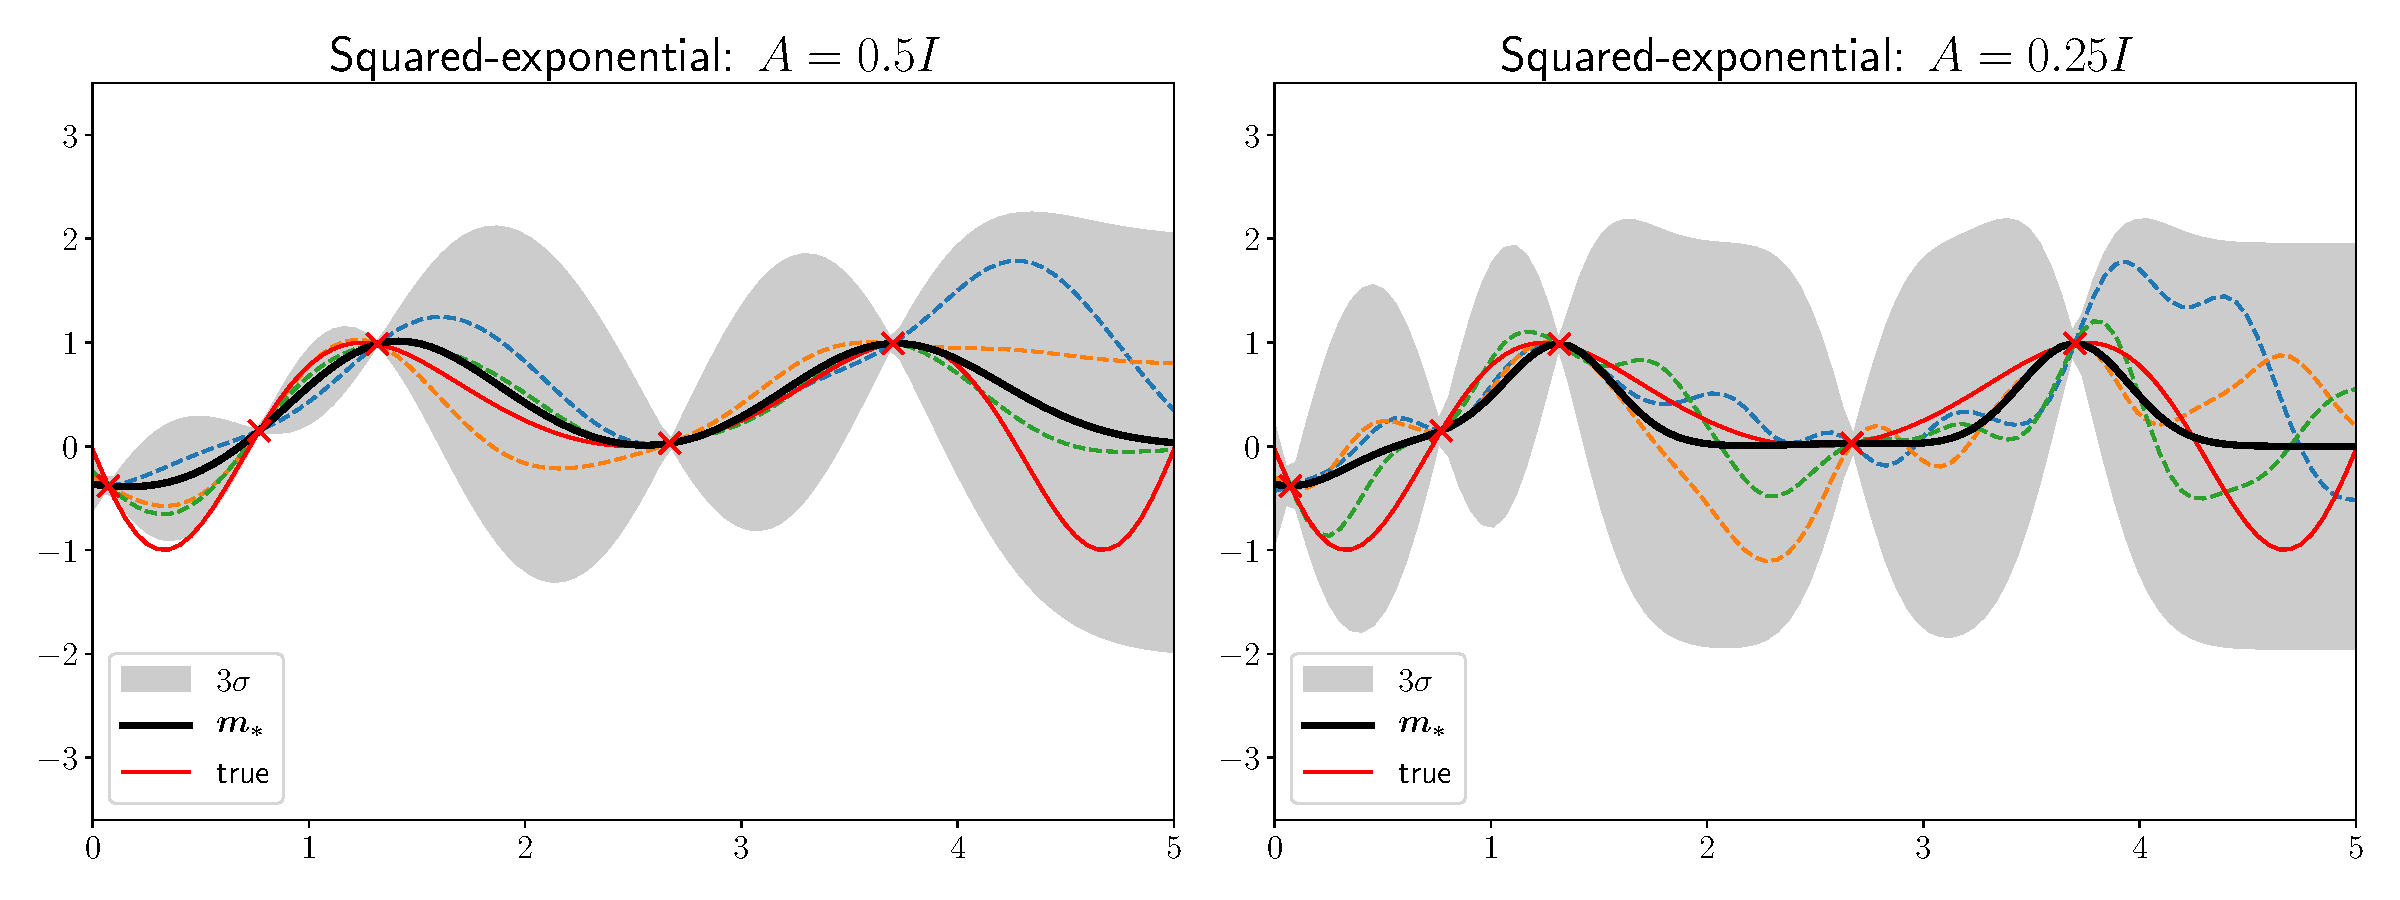
\includegraphics[scale=0.4,center]{SE.pdf}
      \caption{Вид типичных реализаций Гауссовского процесса в зависимости от параметра $A$ функции расстояния для ядра Squared-Exponential}
      \label{fig:se}
\end{figure}

Например, если рассмотреть ядро SE, имеющего колоколообразную форму, то в зависимости от вида функции расстояния будут менять вид типичные реализации Гауссовского процесса.

Квадратично-экспоненциальное ядро (SE):
$$
    k_{SE}(r) = \exp\left(-r^2\right),
$$

% Поскольку ковариационная функция зависит лишь от расстояния между объектами, будем писать $k(d(\cdot, \cdot))$, где $d$ -- некоторая функция расстояния между объектами (например, $d^2(x, x') = (x-x')^TA(x-x'),$ где $A$ -- некоторая настраиваемая диагональная матрица.




Можно также рассматривать более общее семейство ядер Matérn:
$$
    k_{\text{Matérn}}(r) = \frac{2^{1-\nu}}{\Gamma(\nu)}\left( \sqrt{2\nu}r\right)^{\nu}K_{\nu}\left(\sqrt{2\nu}r\right),
$$
где $K_\nu$ -- модифицированная функция Бесселя. Здесь параметр $\nu$ является настраиваемым.
\begin{figure}[h]
    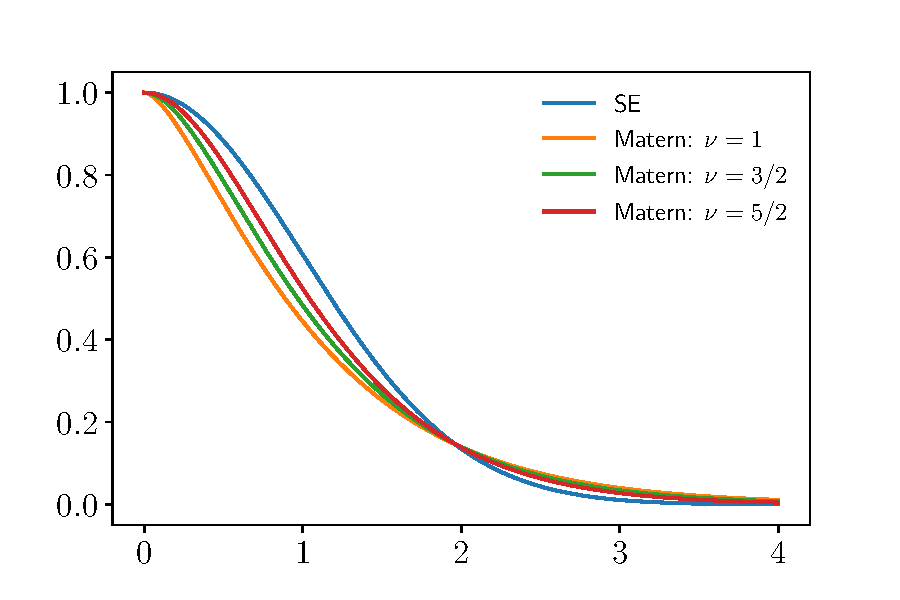
\includegraphics[scale=0.8,center]{diff_kernels.pdf}
      \caption{Различие профилей функций из семейства Matérn}
      \label{fig:diff_kernels}
\end{figure}

На практике обычно фиксируется параметр $\nu = \frac{5}{2}$ или $\nu = \frac{3}{2}$:
$$
    k_{\nu=3/2}(r) = \left(1 + \sqrt{3}r\right)\exp\left(-\sqrt{3}r\right)
$$
$$
    k_{\nu=5/2}(r) = \left(1 + \sqrt{5}r + 5r^2/3\right)\exp\left(-\sqrt{5}r\right)
$$

Также существуют ядра для категориальных гиперпараметров. При этом в качестве функции расстояния можно использовать взвешенное расстояние Хэмминга\cite{10.1007/978-3-642-25566-3_40}:
$$
    k_{cat}(\boldsymbol{\mathrm{x}}_p, \boldsymbol{\mathrm{x}}_q) = \exp\left[\sum_{i=1}^{d} -\lambda_i(1 - \delta(\boldsymbol{\mathrm{x}}^{i}_{p}, \boldsymbol{\mathrm{x}}^{i}_{q}))\right],
$$
где параметры $\lambda_i$ -- настраиваемые, $\delta(\cdot, \cdot)$ -- символ Кронекера. 

Помимо этого можно использовать свойства ядер и строить их композиции:
$$
    k_{mix}(\boldsymbol{\mathrm{x}}_p, \boldsymbol{\mathrm{x}}_q) = k_{\text{Matérn}}(\boldsymbol{\mathrm{x}}_p^{cont}, \boldsymbol{\mathrm{x}}_q^{cont}) + k_{cat}(\boldsymbol{\mathrm{x}}_p^{cat}, \boldsymbol{\mathrm{x}}_q^{cat}), 
$$
где $\boldsymbol{\mathrm{x}}^{cat}$ -- категориальные составляющие вектора гиперпараметров, $\boldsymbol{\mathrm{x}}^{cont}$ -- непрерывные.
Параметры ядра $\theta$ можно настраивать автоматически с помощью максимизации правдоподобия:
$$
    p(\boldsymbol{y}|X, \theta) = \int p(\boldsymbol{y}, \boldsymbol{f} | X, \theta) p(\boldsymbol{f} | X, \theta) d\boldsymbol{f} \longrightarrow \max_{\theta}
$$
Далее обозначим матрицу ковариации, полученное через параметризуемую ковариационную функцию как $K_\theta(X, X)$. Поскольку нормально распределение принадлежит экспоненциальному классу распределений, то интеграл выше может быть выражен аналитически. Тогда, логарифмируя нормальное распределение, имеем равносильную формулировку:
$$
    \log p(\boldsymbol{y} | X, \theta) = -\frac{n}{2} \log({2\pi}) - \frac{1}{2}\log\left(\det\left(K_{\theta}(X, X) + \sigma_n^2I\right)\right) -\frac{1}{2} \boldsymbol{y}^T(K_{\theta}(X, X) + \sigma_n^2I)\boldsymbol{y}
$$
$$
    \log p(\boldsymbol{y} | X, \theta) \longrightarrow \max_{\theta}
$$
Также можно рассмотреть смещенную версию Гауссовского процесса с параметризованной функцией среднего $m_{\theta}$, задающую отступ и аналогично настраивать её параметры.


\subsubsection{Вспомогательные функции}

Пусть выполняется $n$-ая итерация метода, тогда до этого были рассмотрены точки из $\mathcal{D}_n$ и требуется предоставить следующую точку для эксперимента $\boldsymbol{\mathrm{x}}_{n+1}$. Рассмотрим функцию полезности $U : \mathbb{R}^d \times \mathbb{R} \times \Theta \rightarrow \mathbb{R}$. Она показывает качество эксперимента, то есть если бы была рассмотрена тройка $(\boldsymbol{\mathrm{x}}, v, \theta)$, где $\boldsymbol{\mathrm{x}}$ -- рассматриваемая точка, $v = f(x)$ -- соответствующее значение оптимизируемой функции в точке $\boldsymbol{\mathrm{x}}$, $\theta$ -- параметры используемой модели. Тогда, маргинализуя по параметрам $\theta$ и $v$ можно получить ожидаемую полезность точки $\boldsymbol{\mathrm{x}}$:
$$
    \alpha(\boldsymbol{\mathrm{x}}; \mathcal{D}_n) = \E_{\theta}\E_{v| \boldsymbol{\mathrm{x}}, \theta} \left[U(\boldsymbol{\mathrm{x}}, v, \theta)\right].
$$
Далее именно эту функцию будем называть вспомогательной. Обычно при их оптимизации считают, что параметры модели $\theta$ фиксированы.

Существует много различных подходов к выбору функции полезности, рассмотрим некоторые из них.

\paragraph{Подходы, основанные на улучшении}
Предположим, что на текущей итерации лучшим значением является $\tau$ и решается задача максимизации. Тогда в качестве вспомогательной функции можно использовать вероятность улучшения (Probability of improvement). Заметим, что если бы Гауссовский процесс был выбран в качестве вероятностной модели, то вероятность улучшения записывалась как:
$$
    \alpha_{PI}(\boldsymbol{\mathrm{x}}; \mathcal{D}_n) = \mathbb{P}\left[v > \tau\right] = \Phi\left(\frac{\mu_n(\boldsymbol{\mathrm{x}}) - \tau}{\sigma_n(\boldsymbol{\mathrm{x}})}\right),
$$
заметим, что в данном случае $U(\boldsymbol{\mathrm{x}}, v, \theta) = \mathbb{I}\left[v > \tau\right]$, а выбор следующей точки будет соответствовать моде рассматриваемого апостериорного распределения.

Также можно учитывать насколько сильно улучшилось бы значение рассматриваемой функции, в таком случае функцию полезности и соответствующую вспомогательную функцию можно записать в виде:
$$
    U(\boldsymbol{\mathrm{x}}, v, \theta) = (v - \tau)\mathbb{I}\left[v > \tau\right]$$
$$
    \alpha_{EI}(\boldsymbol{\mathrm{x}}; \mathcal{D}_n) = (\mu_n(\boldsymbol{\mathrm{x}}) - \tau)\Phi\left(\frac{\mu_n(\boldsymbol{\mathrm{x}}) - \tau}{\sigma_n(\boldsymbol{\mathrm{x}})}\right) + \sigma_n(\boldsymbol{\mathrm{x}})\phi\left(\frac{\mu_n(\boldsymbol{\mathrm{x}}) - \tau}{\sigma_n(\boldsymbol{\mathrm{x}})}\right),
$$
где $\phi(\cdot)$, $\Phi(\cdot)$ -- соответственно функция плотности и функция распределения стандартного нормального распределения $\mathcal{N}(0, 1)$. Данная вспомогательная функция показывает ожидаемое улучшение (Expected-Improvement).

\paragraph{Подходы, основанные на оптимистическом предсказании} 
В данном случае предполагается, что прогноз модели будет соответствовать оптимистичному варианту. Примером вспомогательной функции для такого подхода является верхняя граница гауссовского процесса (Gaussian process upper confidence bound): 

$$
     \alpha_{UCB}(\boldsymbol{\mathrm{x}}; \mathcal{D}_n) = 
     \mu_n(\boldsymbol{\mathrm{x}}) + \sqrt{\beta_n}\sigma_n(\boldsymbol{\mathrm{x}}), 
$$
здесь параметр $\beta_n$ -- настраиваемый. 

\paragraph{Подходы, использующие информационную ценность}

В данном случае учитываются апостериорные распределения по неизвестному минимизатору $\boldsymbol{\mathrm{x^{*}}}$. Далее будем его обозначать как $p_{*}(\boldsymbol{\mathrm{x}} | \mathcal{D}_{n})$. Такие распределения неявно индуцируются апостериорными распределением на целевую переменную $f$.
Рассмотрим используемого здесь метода -- entropy serach (ES), главной задачей которого является уменьшение неопределённости в положении $\boldsymbol{\mathrm{x^{*}}}$. В терминах функции полезности будем записывать это как:
$$U(\boldsymbol{\mathrm{x}}, y, \theta) = H(\boldsymbol{\mathrm{x^{*}}} | \mathcal{D}_n) - H(\boldsymbol{\mathrm{x^{*}}} | \mathcal{D}_n \cap \{(x, y)\},$$
где $H(\cdot)$ -- это дифференциальная энтропия апостериорного распределения $p_{*}(\boldsymbol{\mathrm{x}} | \mathcal{D}_{n})$. Тогда вспомогательная функция будет иметь вид:
$$
    \alpha_{ES}(\boldsymbol{\mathrm{x}} ; \mathcal{D}_{n}) = H(\boldsymbol{\mathrm{x^{*}}} | \mathcal{D}_n) - \E_{y | \mathcal{D}_n, \boldsymbol{\mathrm{x}}} H(\boldsymbol{\mathrm{x^{*}}} | \mathcal{D}_n \cup \{(x, y)\}),\; y \sim \mathcal{N}(\mu_n(\boldsymbol{\mathrm{x}}), \sigma_n^2(\boldsymbol{\mathrm{x}}) + \sigma^2).
$$
Но поскольку данная функция непригодна для непрерывных областей поиска используется другой вариант записи для данной вспомогательной функции (Predictive Entropy Search):
$$
\alpha_{PES}(\boldsymbol{\mathrm{x}} ; \mathcal{D}_{n}) = H(y | \mathcal{D}_n, \boldsymbol{\mathrm{x}}) - \E_{ \boldsymbol{\mathrm{x^{*}}} | \mathcal{D}_n} H(y | \mathcal{D}_n, \boldsymbol{\mathrm{x^{*}}}, \boldsymbol{\mathrm{x^{*}}}),
$$
здесь было использовано свойство симметричности для взаимной информации. В работе \cite{hernndezlobato2014predictive} указаны эффективные методы вычисления данного выражения.

\subsubsection{Tree Parazen Estimators}

Рассмотрим другую вероятностную модель \cite{NIPS2011_4443}, которая в отличие от Гауссовского процесса, где апостериорное распределение на  функцию отклика $p(f|\boldsymbol{\mathrm{x}})$ формируется напрямую, моделирует это распределение через $p(\boldsymbol{\mathrm{x}}|f)$ и $p(f)$. В данном случае структурное пространство гиперпараметров описывается с помощью дерева. В каждом узле оно подменяет $p(x|y)$ непараметрическими распределениями, вид которых определяется видом гиперпараметра. Например, равномерное распределение заменяется усечённой смесью гауссиан, категориальное -- перевзвешенным категориальным. Таким образом имеем:
$$
    p(\boldsymbol{\mathrm{x}}|f, \mathcal{D}) = \begin{cases}
        l(\boldsymbol{\mathrm{x}}) \quad &\text{если } f < f^{*}, \\
        g(\boldsymbol{\mathrm{x}}) \quad &\text{если } f \geqslant f^{*},
    \end{cases}
$$
где $f^{*}$ -- лучшее наблюдаемое значение минимизируемой функции $f$, а $l(\cdot)$, $g(\cdot)$ -- заменяющие распределения. Далее фиксируется некоторая квантиль $\gamma$, такая что $P(f < f^{*}) = \gamma$ -- условно <<мягкость>> модели, чтобы модель могла сэмплировать точки из $g(\boldsymbol{\mathrm{x}})$. На априорное распределения $p(y)$ ограничения не накладываются. 

Тогда можно записать выражение для:

\begin{equation*}
    \alpha_{EI} = \int_{-\infty}^{f^{*}} (f^{*} - f) p(f|x)\, df =  \int_{-\infty}^{f^{*}} (f^{*} - f) \frac{p(\boldsymbol{\mathrm{x}} | f) p(f)}{p(\boldsymbol{\mathrm{x}})} \,df = \frac{\gamma f^{*}l(\boldsymbol{\mathrm{x}}) - l(\boldsymbol{\mathrm{x}}) \int_{-\infty}^{f^{*}} [fp(f)] \,df}{\gamma l(\boldsymbol{\mathrm{x}}) + (1-\gamma)g(\boldsymbol{\mathrm{x}})}.
\end{equation*}
Заметим, что:
$$
    \alpha_{EI} \propto \left(\gamma + \frac{g(\boldsymbol{\mathrm{x}})}{l(\boldsymbol{\mathrm{x}})}(1-\gamma)\right)^{-1},
$$
откуда следует, что для того чтобы максимизировать $\alpha_{EI}$, алгоритму будет выгоднее брать точки для которых отношение $g(\boldsymbol{\mathrm{x}}) / l(\boldsymbol{\mathrm{x}})$ минимально. 

% Например, в качестве таковой функции может быть  использована верхняя граница уверенности гауссовского процесса (Gaussian process upper confidence bound rule):
% $$\phi_t(x) = \mu_{t-1}(x) + \beta_t^{1/2}\sigma_{t-1}(x),$$
% здесь $\mu_{t-1}(x), \sigma_{t-1}(x)$ --- это апостериорное среднее и стандартное отклонение гауссовского процесса после $t-1$ шага. Параметр $\beta_{t}^{1/2}$ задаёт коэффициент разведки и использования. Или же можно использовать в качестве вспомогательной функции ожидаемое улучшение:
% $$\E{\mathcal{I}(\lambda)} = \E{\max(f_{min} - y, 0)},$$
% здесь $f_{min}$ -- ранее найденный минимум, $y$ -- предполагаемое значение функции.

% Если параметр конфигурации $\lambda$ задаёт нормальное распределение на предпологаемое значение функции $y \sim \mathcal{N}(\mu(\lambda), \sigma^2)$, то значение ожидаемого улучшения можно вычислить по следующей формуле:
% $$\E{\mathcal{I}(\lambda)} = \left(f_{min} - \mu(\lambda)\right) \Phi\left(\frac{f_{min} - \mu(\lambda)}{\sigma}\right) + \sigma\phi\left(\frac{f_{min} - y}{\sigma}\right), $$
% где $\phi(\cdot)$, $\Phi(\cdot)$ -- соответственно функция плотности и функция распределения стандартного нормального распределения $\mathcal{N}(0, 1)$.

% [[[[[Prediction of improvement, Thompson Sampling, Entropy Search]]]]]

\section{Эксперименты}
	Предлагается сравнить представленные выше методы на качество и скорость работы. В данном случае под скоростью понимается количество итераций нужное для сходимости до примерного глобального минимума в сравнении с другими методами. Сравнение времени работы реализаций методов, используемых автором, с технической точки зрения было бы некорректным. Методы GP-EI, GP-PI, GP-UCB, TPE-EI исполняются, не используя промежуточных фаз, прямо из Python. Spearmint рассматривает каждую итерацию GP-PES как отдельную задачу, причём для каждой создаётся отдельный процесс. После этого данные заносятся в базу данных MongoDB. С учётом этого сравнение времени будет подразумевать сравнение верхних временных границ, которые могут сильно отличаются от точных значений. 
	
	Предлагается рассмотреть работу данных алгоритмов на функциях из стандартного набора для тестирования оптимизационных методов \cite{simulationlib} и при подборе оптимальных параметров SVM, обучаемого на датасете MNIST \cite{lecun-mnisthandwrittendigit-2010}. В таблице \ref{tab:func} и на рисунке \ref{tab:func} представлены рассматриваемые функции.
	
	\newpage
	
		\begin{table}[h]
		\begin{center}
			\begin{tabular}{|c|c|} 
				\hline
				Метод & Реализация \\ [0.5ex] 
				\hline\hline
				GP-PI, GP-EI, GP-UCB & Scikit-Optimize \cite{ScikitOptimizeCode} \\ 
				\hline
				GP-PES & Spearmint \cite{SpearmintCode} \\
				\hline
				TPE-EI & HyperOpt \cite{HyperoptCode} \\
				\hline
			\end{tabular}
			\caption{\label{tab:real} Реализации методов.}
		\end{center}
	\end{table}
	

	
	\begin{table}[h!]
		\begin{center}
			\begin{tabular}{|c|c|c|} 
				\hline
				Название & Функциональное представление& Минимальное значение \\ 
				и рассматриваемя область& & и точки оптимума \\
				[0.5ex] 
				\hline\hline
				
				Branin Function & $f(\boldsymbol{\mathrm{x}}) = (x_2 - \frac{5.1}{4\pi^2}x_1^2 + \frac{5}{\pi}x_1 - 6)^2+$ & $f(\boldsymbol{\mathrm{x_{*}}}) = 0.397887$\\
				$\boldsymbol{\mathrm{x}} \in [-5, 10] \times [0, 15]$& $ + 10(1-\frac{1}{8\pi} \cos{(x_1)})$& $\boldsymbol{\mathrm{x_{*}}} \in \{(9.42478, 2.475),$\\
				& &  $(\pi, -12.275), (-\pi, 12.275)\}$\\
				\hline
				Six-Hump Camel Function & $f(\boldsymbol{\mathrm{x}}) = (4 - 2.1x_1^2 + \frac{x_1^4}{3})x_1^2 + $& $f(\boldsymbol{\mathrm{x_{*}}}) = -1.0316$ \\
				$\boldsymbol{\mathrm{x}} \in [-3, 3] \times [-2, 2]$& $ + x_1x_2  + (-4 + 4x_2^2)x_2^2$ & $\boldsymbol{\mathrm{x_{*}}} \in \{(0.0898, -0.7126),$ \\
				& &  $(0.0898, -0.7126)\}$\\
				\hline
				Rosenbrock Function&$f(\boldsymbol{\mathrm{x}}) = \sum_{i=1}^{d-1}[100(x_{i+1} - x_i^2)^2 +$ &$f(\boldsymbol{\mathrm{x_{*}}}) = 0$ \\
				$\boldsymbol{\mathrm{x}} \in [-5, 10]^d,\; d=2$&  $+ (x_i - 1)^2$ & $\boldsymbol{\mathrm{x_{*}}} = (1, 1, \dots, 1)$\\
				\hline
				Colville Function&$f(\boldsymbol{\mathrm{x}}) = 100(x_1^2 -x_2)^2 + $&$f(\boldsymbol{\mathrm{x_{*}}}) = 0$ \\
				$\boldsymbol{\mathrm{x}} \in [-10, 10]^4$&$+(x_1-1)^2 +(x_3-1)^2 + $&$\boldsymbol{\mathrm{x_{*}}} = (1, 1, \dots, 1)$\\
				&$+90(x_3^2-x_4)^2 + 10.1((x_2-1)^2 +$&\\
				&$+(x_4-1)^2) + 19.8(x_2-1)(x_4-1)$&\\
				\hline
				Easom function & $f(\boldsymbol{\mathrm{x}}) = -\cos{(x_1)}\cos{(x_2)}\times$ & $f(\boldsymbol{\mathrm{x_{*}}}) = -1$ \\
				$\boldsymbol{\mathrm{x}} \in [-100, 100]^2$ & $\times\exp{(-(x_1-\pi)^2-(x_2-\pi)^2)}$ &$\boldsymbol{\mathrm{x_{*}}} =(\pi, \pi)$\\
				\hline
				Griewank Function & $f(\boldsymbol{\mathrm{x}}) = \sum_{i=1}^{d}\frac{x_i^2}{4000} - \prod_{i=1}^{d}\cos{\left(\frac{x_i}{\sqrt{i}}\right)} + 1 $& $f(\boldsymbol{\mathrm{x}}) = 0$\\
				$\boldsymbol{\mathrm{x}} \in [-2, 2]^d, \; d=6$&& $\boldsymbol{\mathrm{x_{*}}} = (0, 0, \dots, 0)$ \\
				\hline
				
			\end{tabular}
			\caption{\label{tab:func} Тестовые функции.}
		\end{center}
	\end{table}

	\begin{figure}[!h]
		\centering
		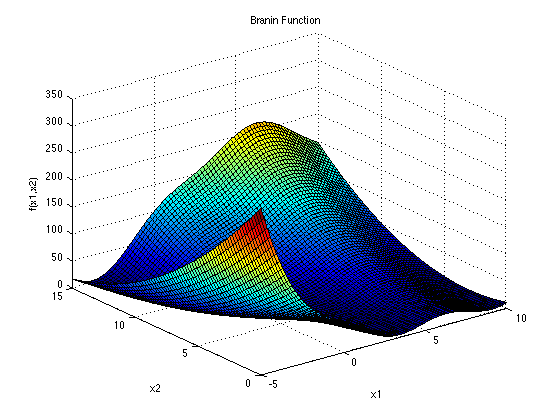
\includegraphics[width=0.5\linewidth]{test_functions/Branin.png}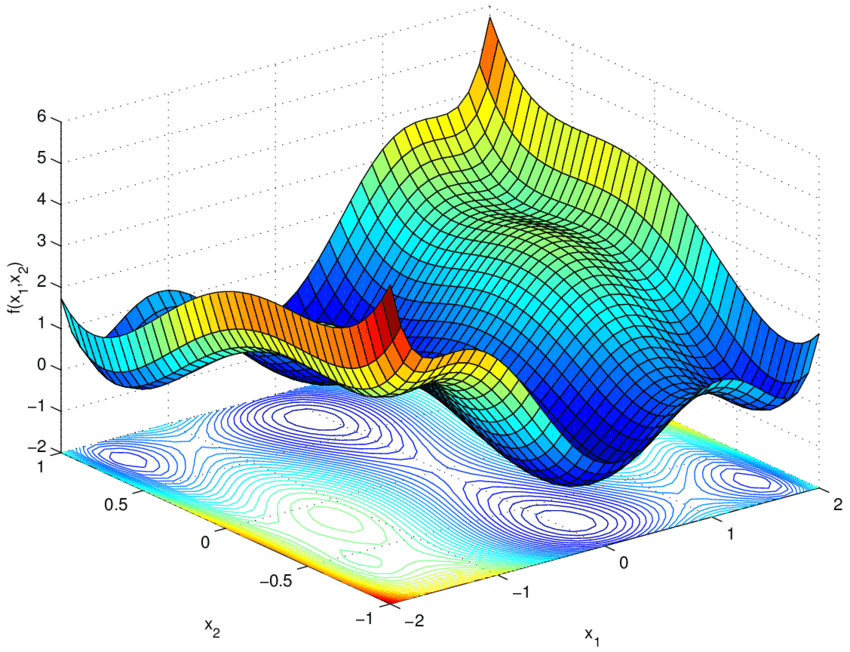
\includegraphics[width=0.5\linewidth]{test_functions/SixHump.png}
		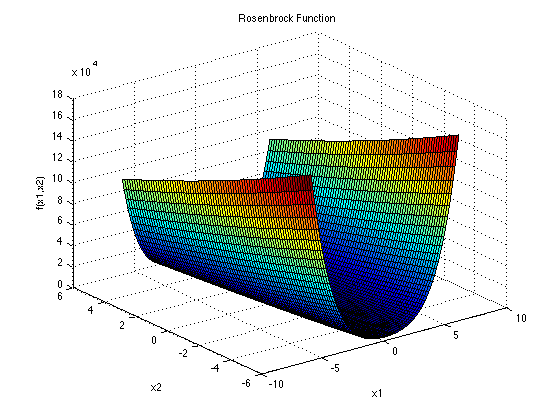
\includegraphics[width=0.5\linewidth]{test_functions/Rosenbrock.png}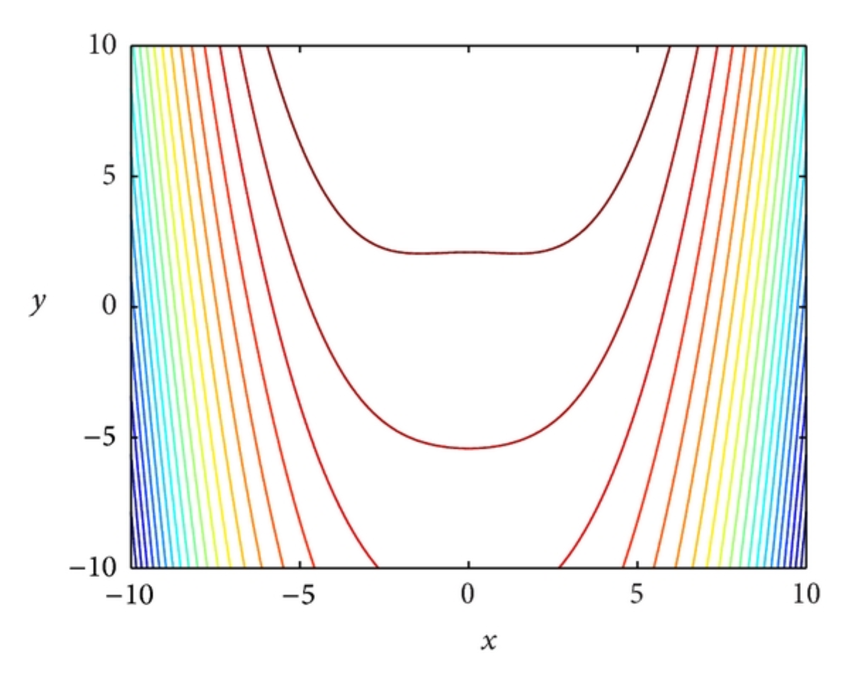
\includegraphics[width=0.5\linewidth]{test_functions/Colville.png}
		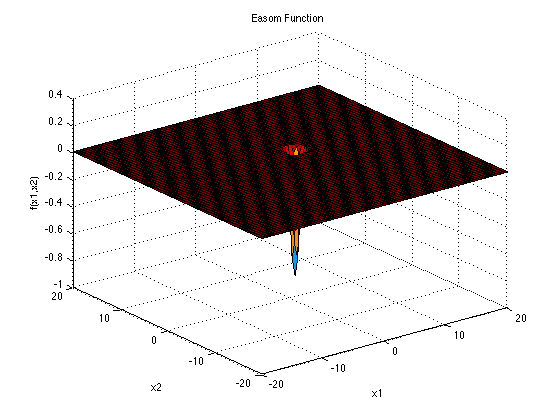
\includegraphics[width=0.5\linewidth]{test_functions/Easom.png}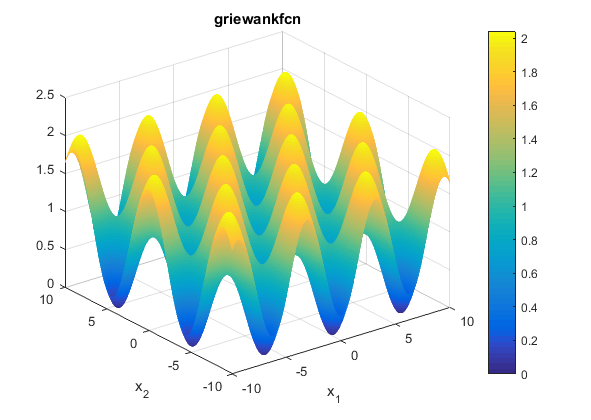
\includegraphics[width=0.5\linewidth]{test_functions/Griewank.png}
		\caption{Графики тестовых функций. Слева направо, сверху вниз это Rosenbrock Function, Six~Hump~Camel~Function, Rosenbrock Function, Colville Function (линии уровня при $x_1 = x_3,\; x_2 = x_4$), Easom Fucntion, Griewank Function (при $d=2$).}
	\end{figure}

	\newpage 
	\subsection{Эксперимент 1}
	Предлагается рассмотреть следующий сценарий: провести сравнение методов, основанных на гауссовском процессе в зависимости от вспомогательной функции. Рассматривались функции: PI, ES, UCB ($\sqrt{\beta_n} = 1.96 = \mathit{const}$ -- значение предлагаемое пакетом Scikit-Optimize по-умолчанию), PES. В данном эксперименте проводились вычисления на некоторых функциях из тестового набора, а также на их зашумлённых версиях. Использовался стандартный Гауссовский шум с параметрами $\mathcal{N}(0, 0.1)$ (моделям сообщалось соответствующее распределение). В качестве ядра Гауссовского процесса рассматривалось настраиваемое с помощью максимизации правдоподобия ядро Matérn 5/2. Вычислительные результаты представлены для 40 итераций соответствующего метода представлены на рисунках \ref{fig:exp1_branin}, \ref{fig:exp1_hump}, \ref{fig:exp1_rosenbrock}, \ref{fig:exp1_griewank}.
	
	В данном случае хуже всего с точки зрения и скорости и качества показала себя UCB. Если функция имеет слишком широкую область значений (как в стучае с Rosenbrock) метод даже не может приблизится к значению оптимума, а остаётся постоянным (параметр $\sqrt{\beta_n}$ -- выбран слишком маленьким). Этого недостатка лишена функция PES, которая как раз-таки хорошо работает на таких функциях, даже при наличии шума (правда, в данном случае он существенен только при приближении к глобальному минимуму функции).
	
	В представленных примерах функции EI и PI работали примерно схоже. Если их сравнивать, то можно видеть, что функция PI работает менее агрессивно (траектория почти гладкая).
	
	Если сравнивать левые и правые графики, то они примерно одинаковы, хотя, это немного странно, если смотреть на вид функций (слишком резко меняются).
	
	\begin{figure}[!h]
		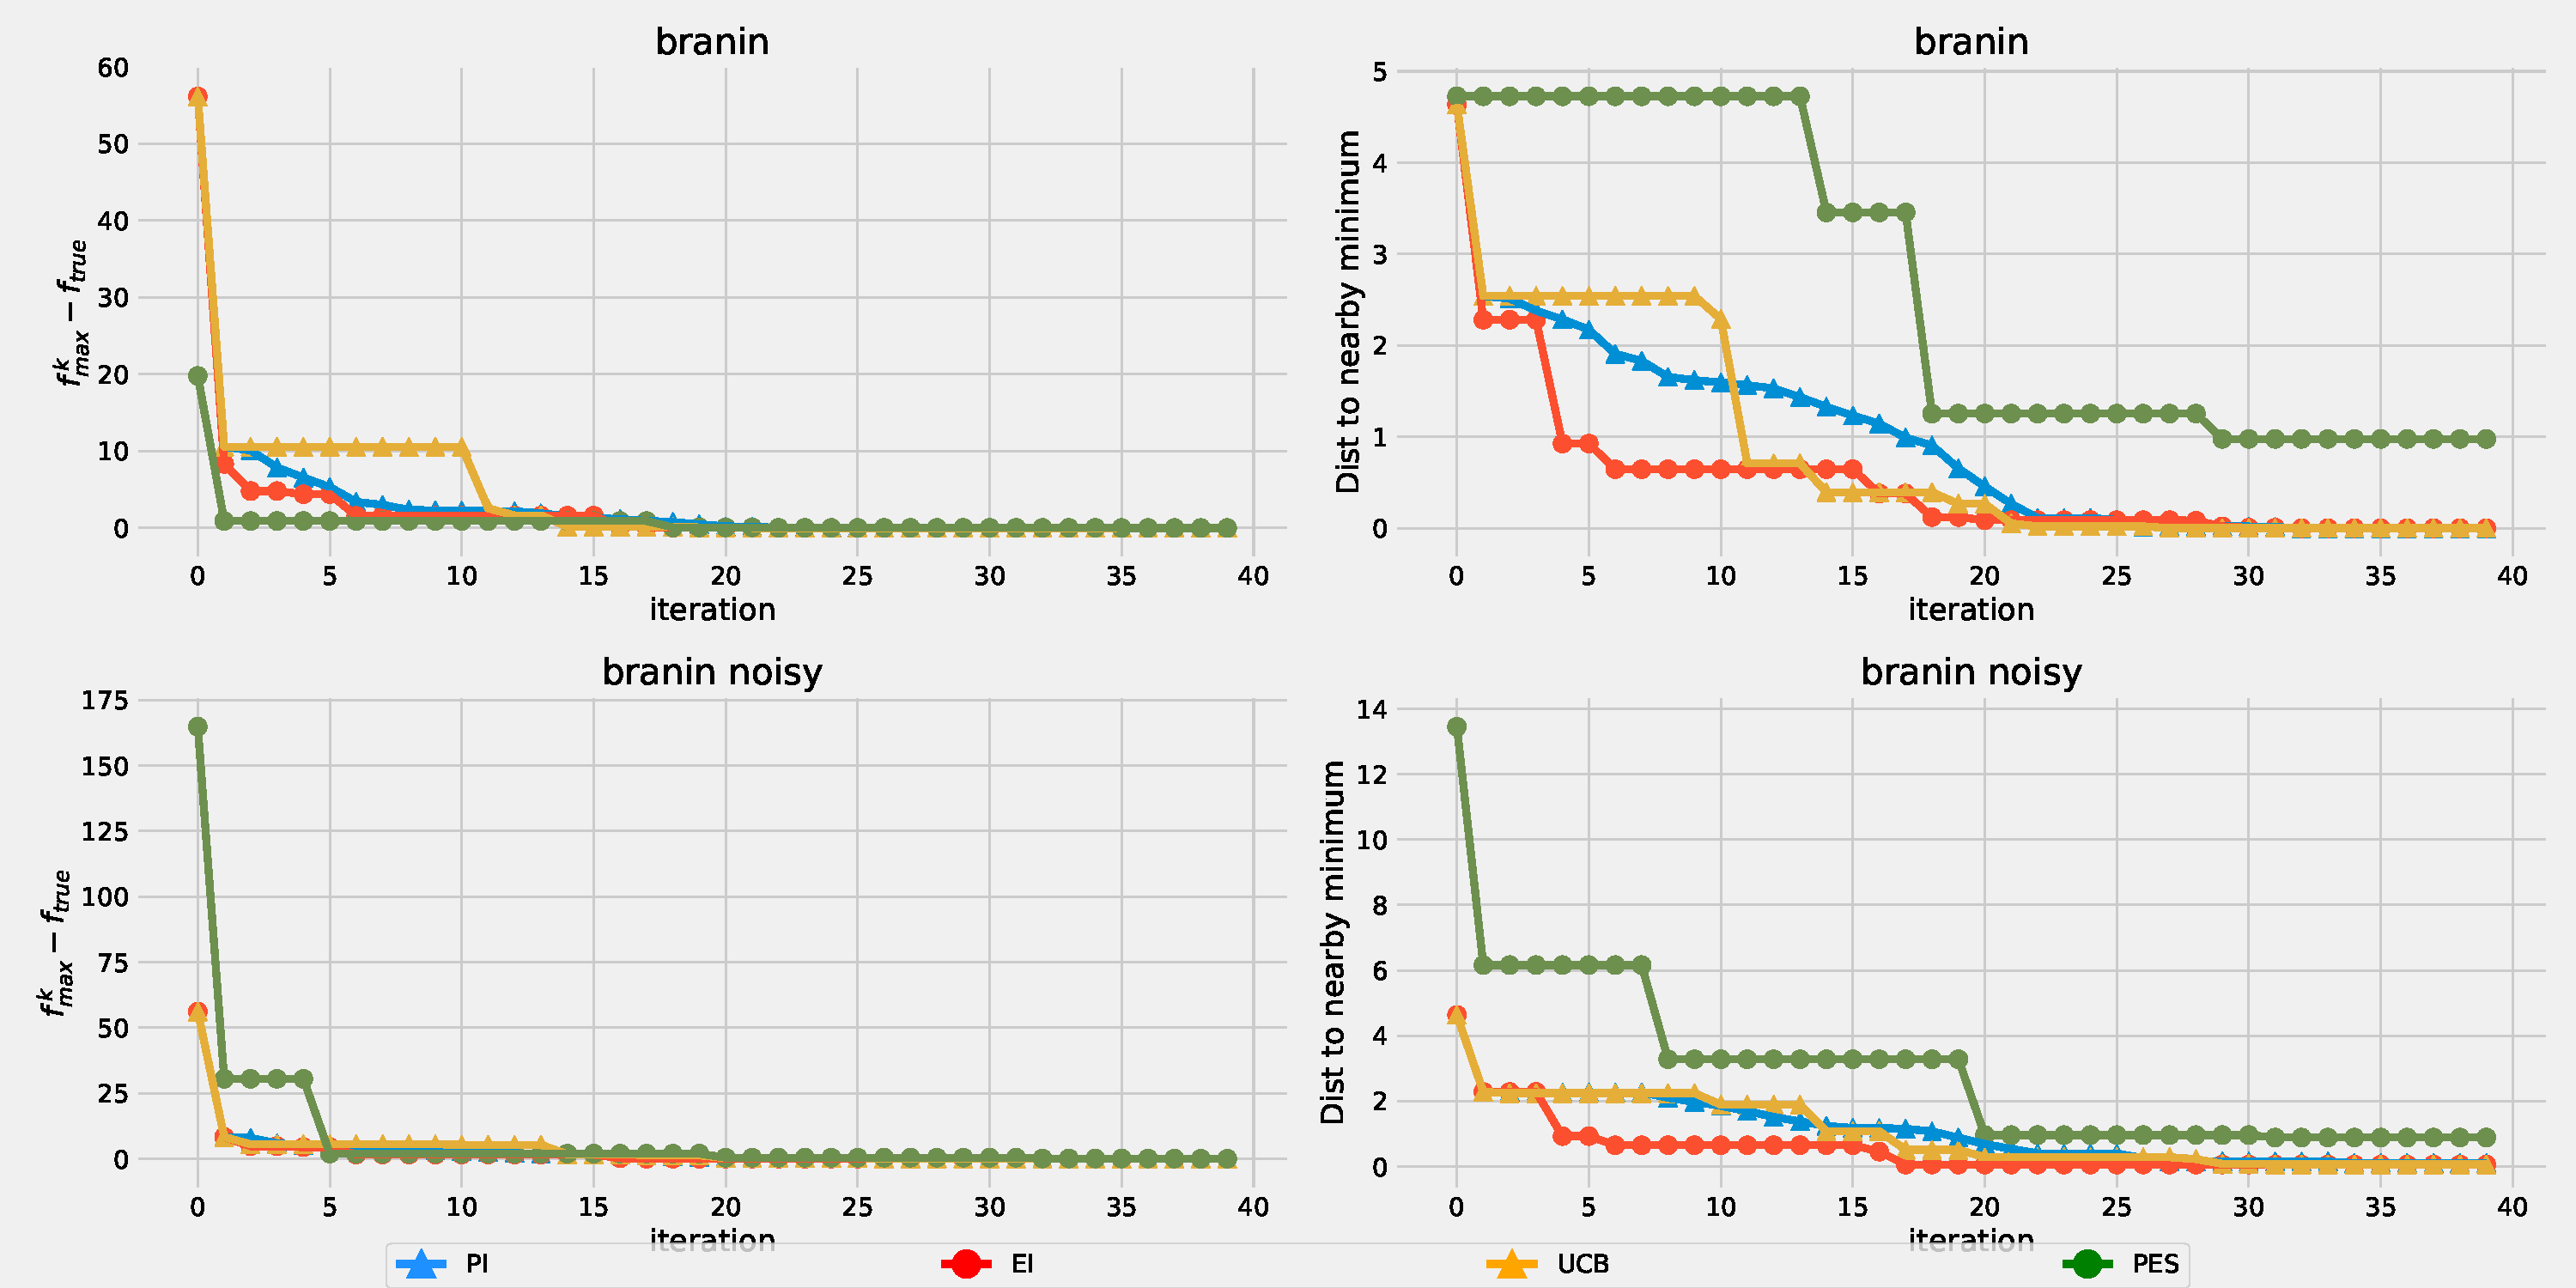
\includegraphics[scale=0.25,center]{../code/exp1/branin.pdf}
		\caption{\textbf{Эксперимент 1:} Branin Function}
		\label{fig:exp1_branin}
	\end{figure}
	
	\begin{figure}[!h]
		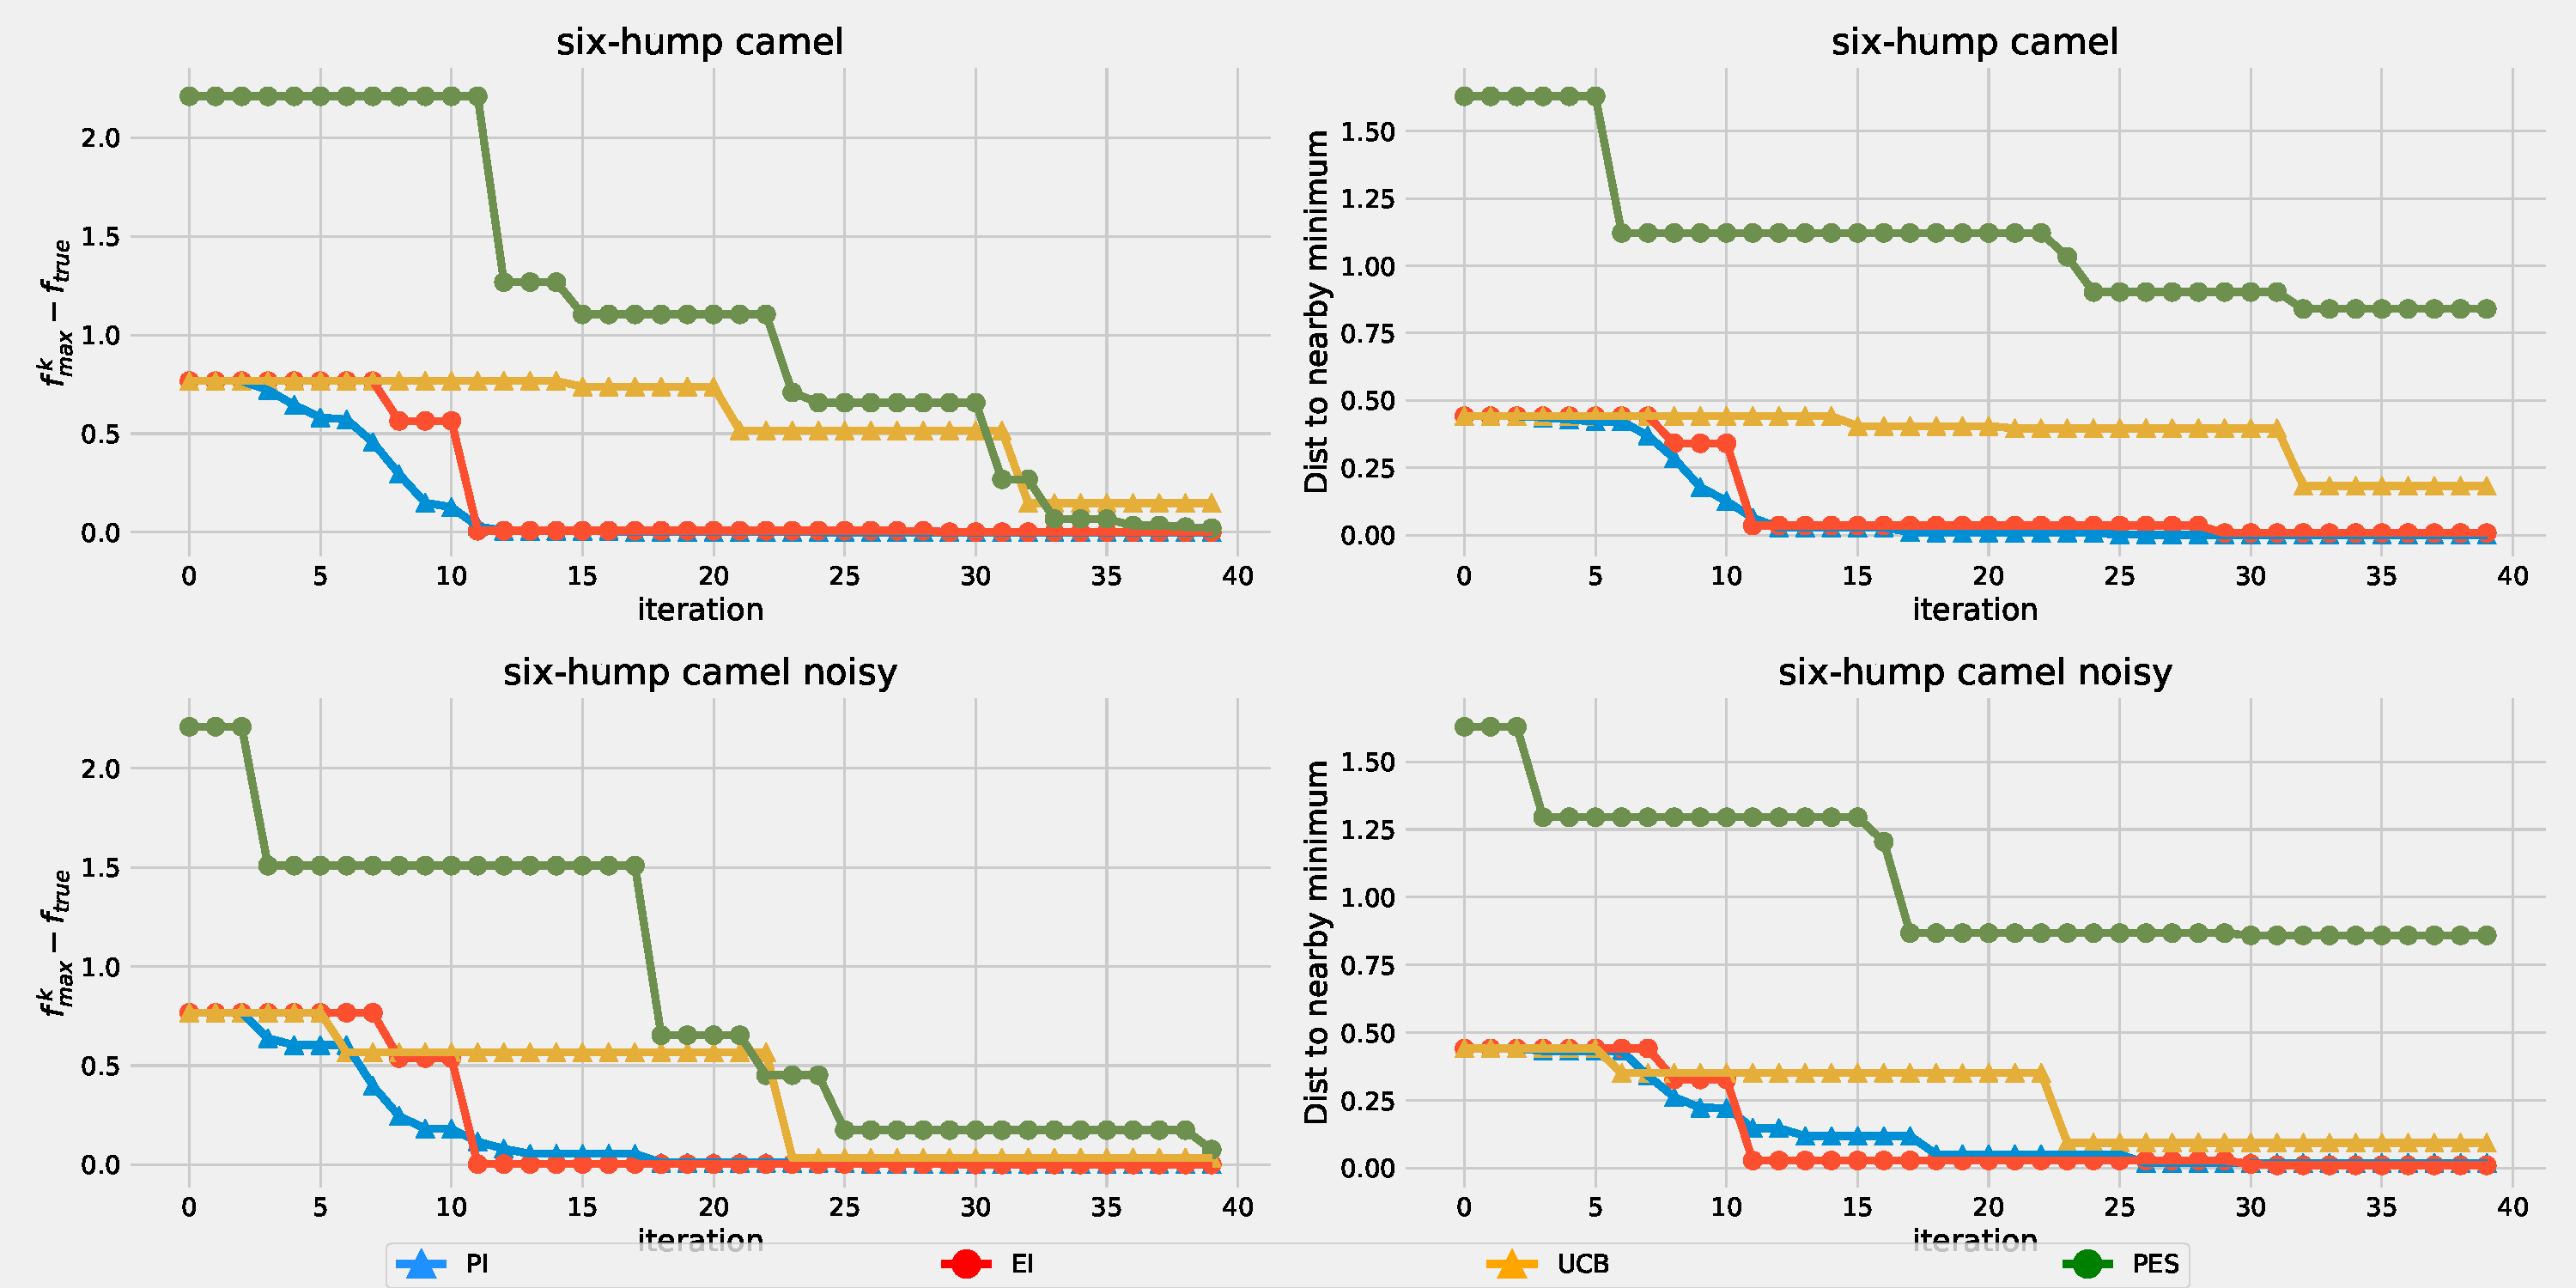
\includegraphics[scale=0.25,center]{../code/exp1/hump.pdf}
		\caption{\textbf{Эксперимент 1:} Six-Hump Camel Function}
		\label{fig:exp1_hump}
	\end{figure}

	\begin{figure}[!h]
		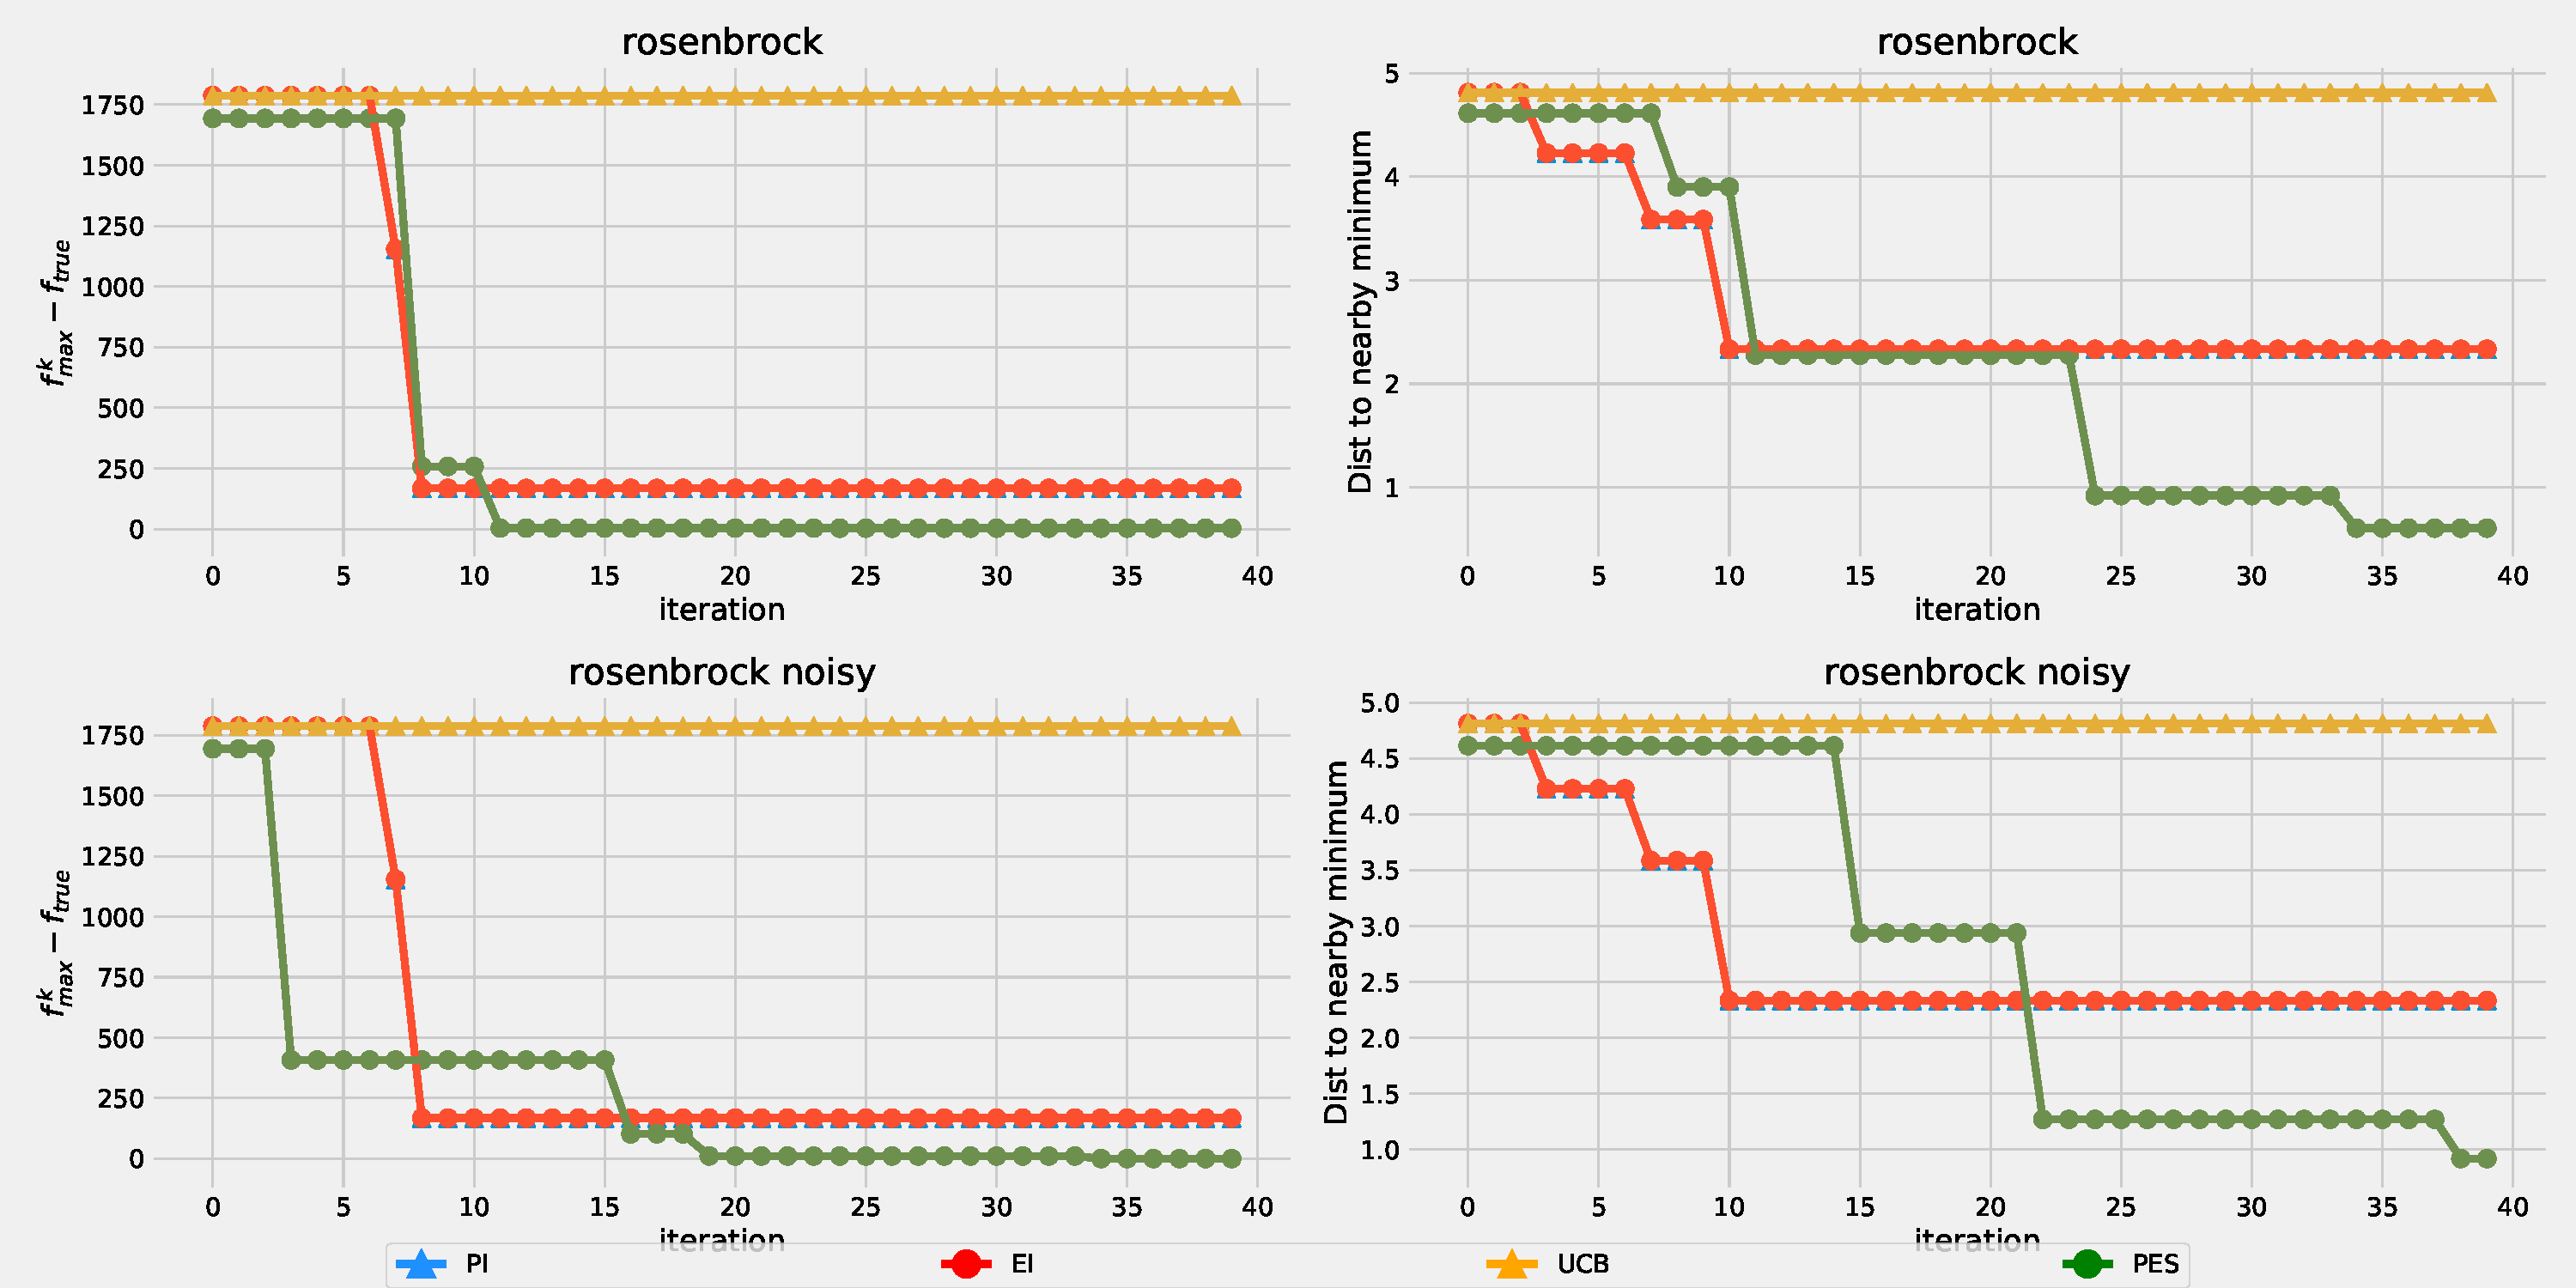
\includegraphics[scale=0.25,center]{../code/exp1/rosenbrock.pdf}
		\caption{\textbf{Эксперимент 1:} Rosenbrock Function}
		\label{fig:exp1_rosenbrock}
	\end{figure}
	
	\begin{figure}[!h]
		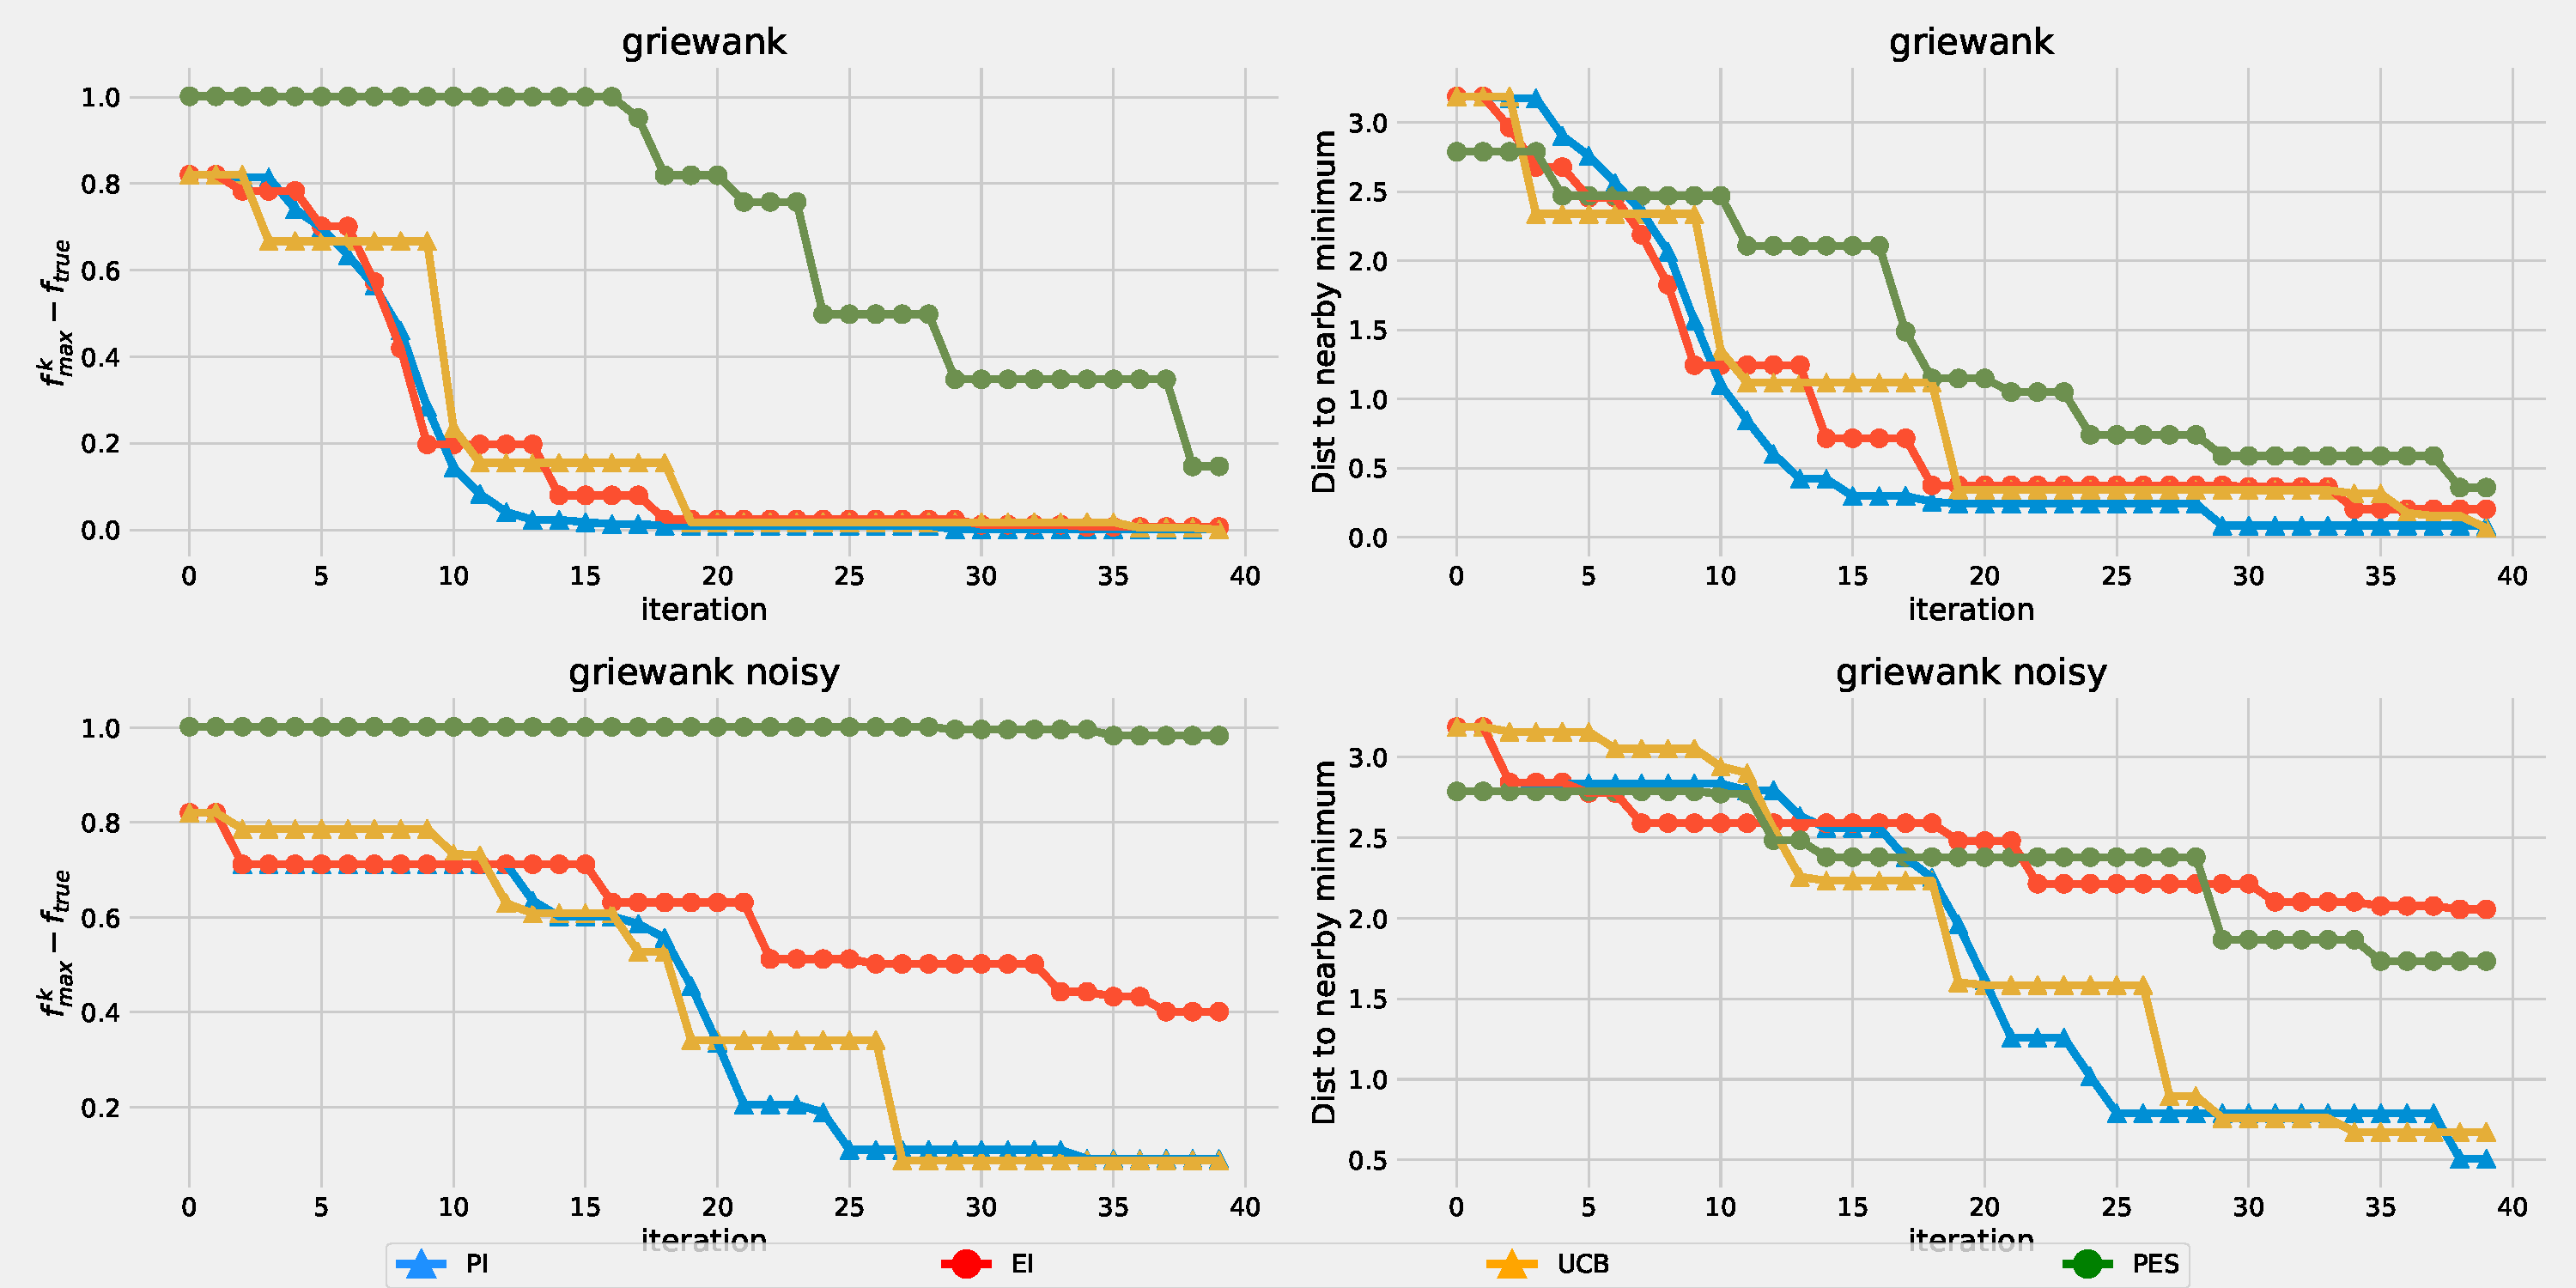
\includegraphics[scale=0.25,center]{../code/exp1/griewank.pdf}
		\caption{\textbf{Эксперимент 1:} Griewank Function}
		\label{fig:exp1_griewank}
	\end{figure}
	

	
	\newpage
	\subsection{Эксперимент 2}
	Предлагалось сравнить подходы в зависимости от структуры, строящегося вероятностного пространства. В качестве вспомогательной функции была взята Expected~Improvement. В данном случае рассматривались следующие комбинации TPE-EI и GP-EI (с настраиваемым ядром  Matérn 5/2). Результаты представлены на рисунках \ref{fig:exp2_branin}, \ref{fig:exp2_griewank}, \ref{fig:exp2_hump}, \ref{fig:exp2_rosenbrock}. 
	В данном случае нельзя выделить лучший метод. TPE-EI чаще меняет свои значения и чаще ближе к значению минимума в сравнении с GP-EI. Однако, метод GP-EI более устойчив к наличию шума в данных.

	\begin{figure}[!h]
		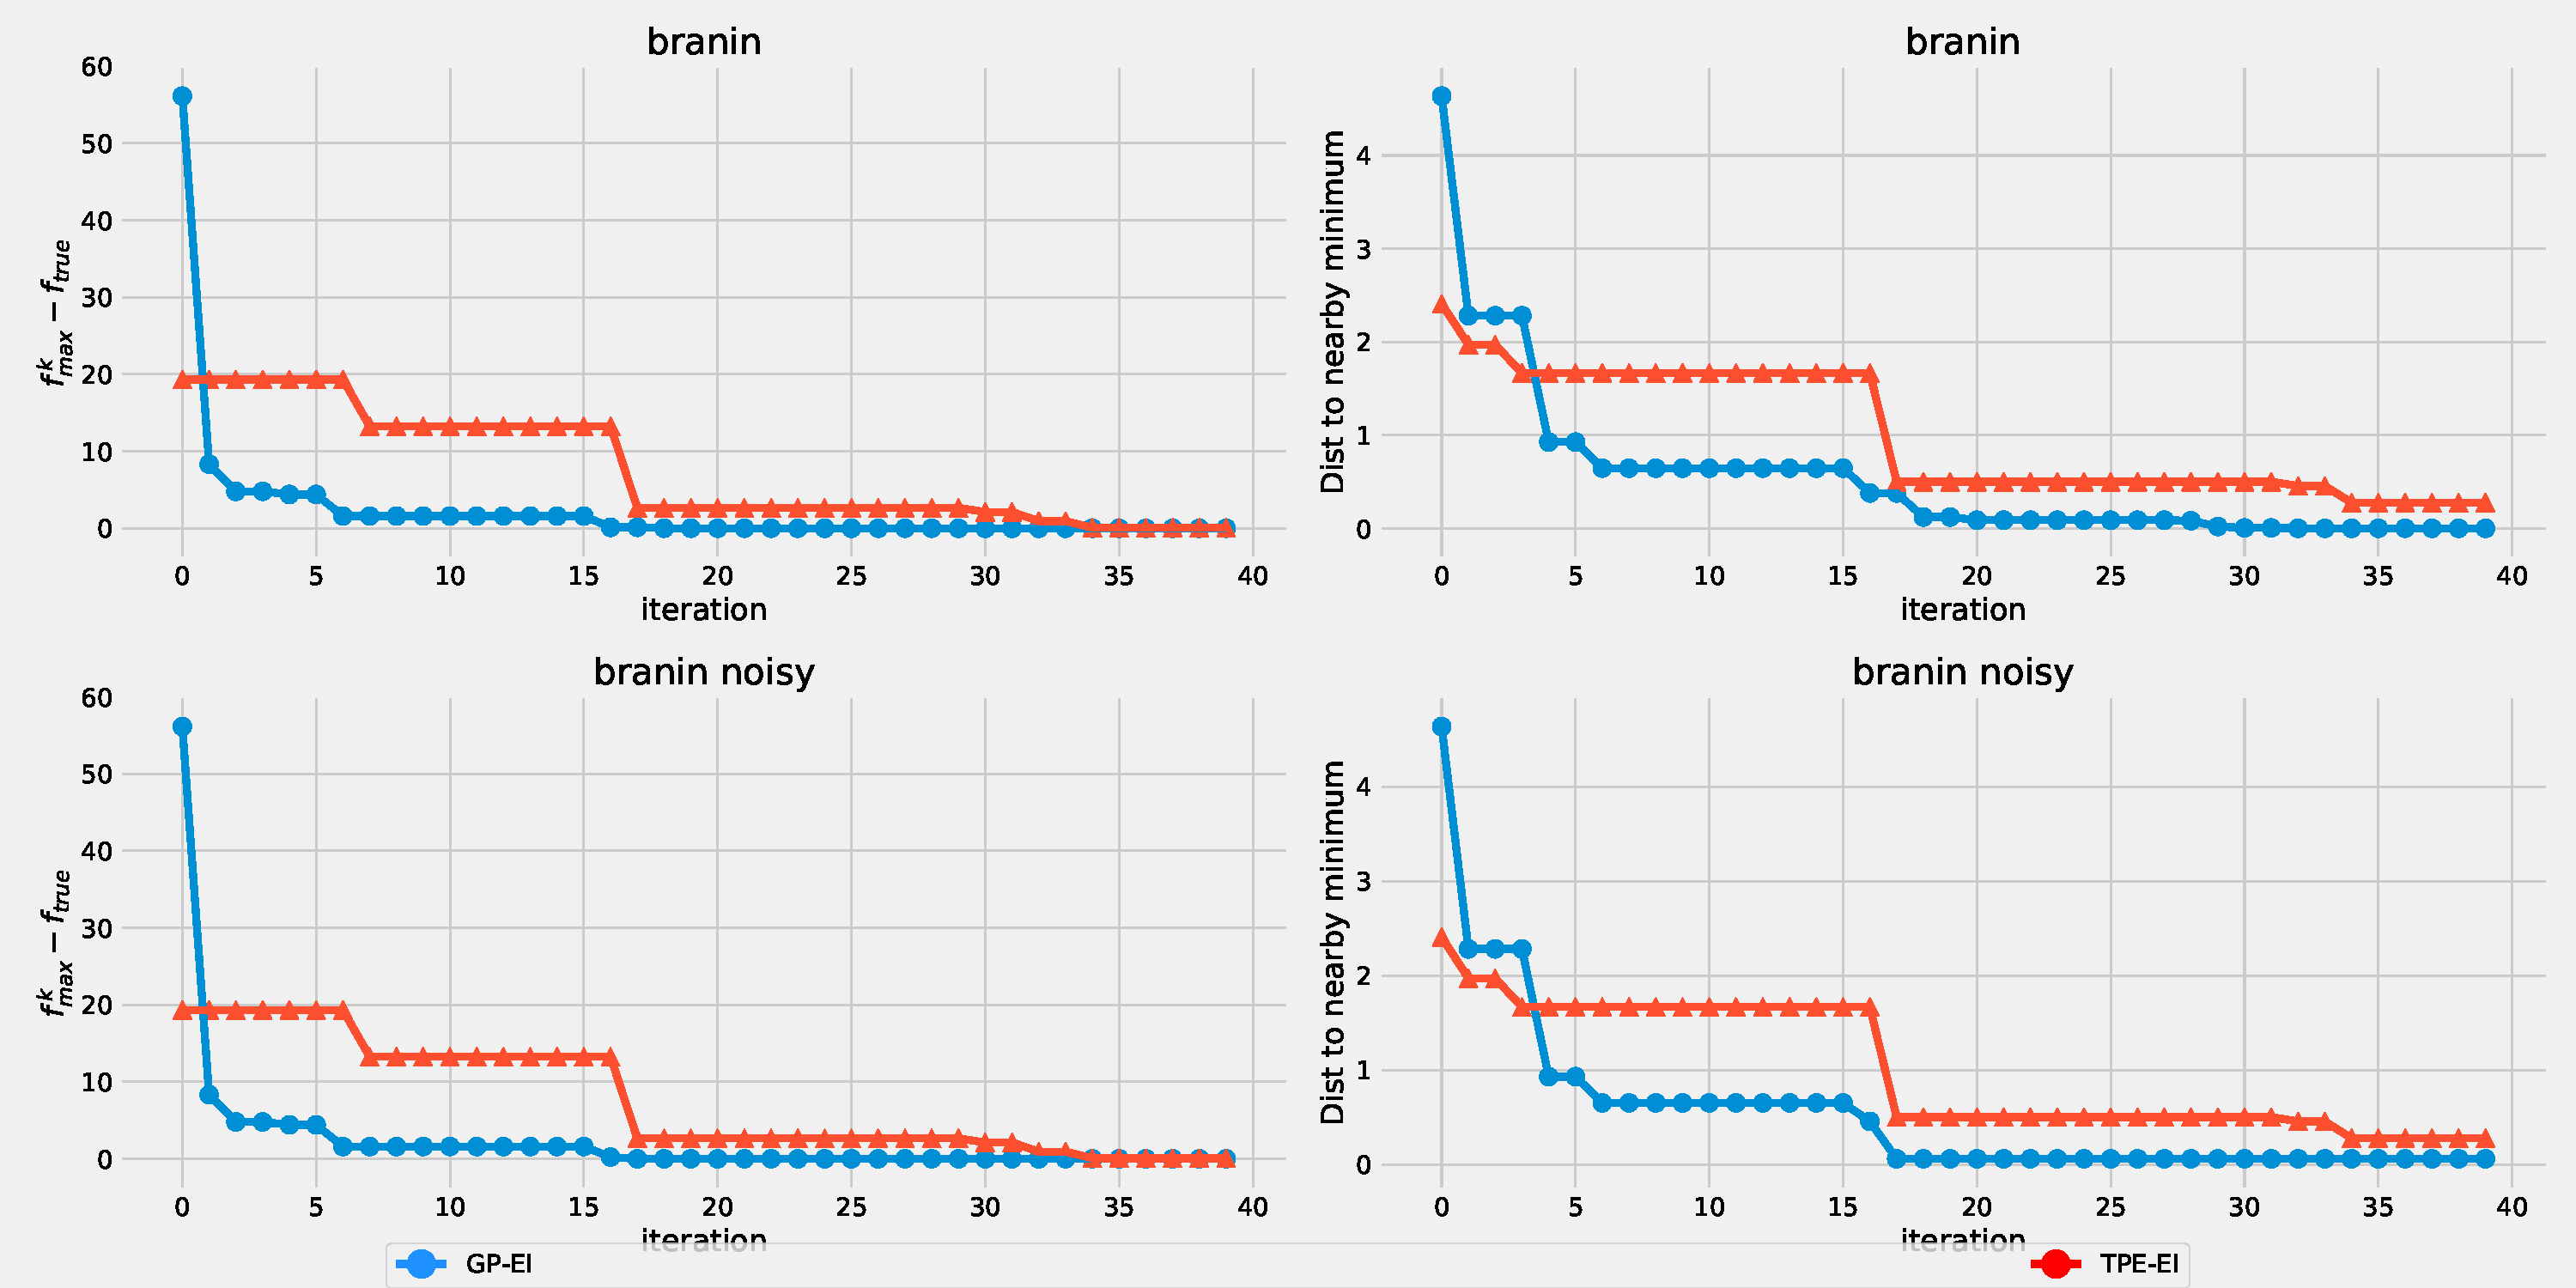
\includegraphics[scale=0.25,center]{../code/exp2/branin.pdf}
		\caption{\textbf{Эксперимент 2:} Branin Function}
		\label{fig:exp2_branin}
	\end{figure}
	
	\begin{figure}[!h]
		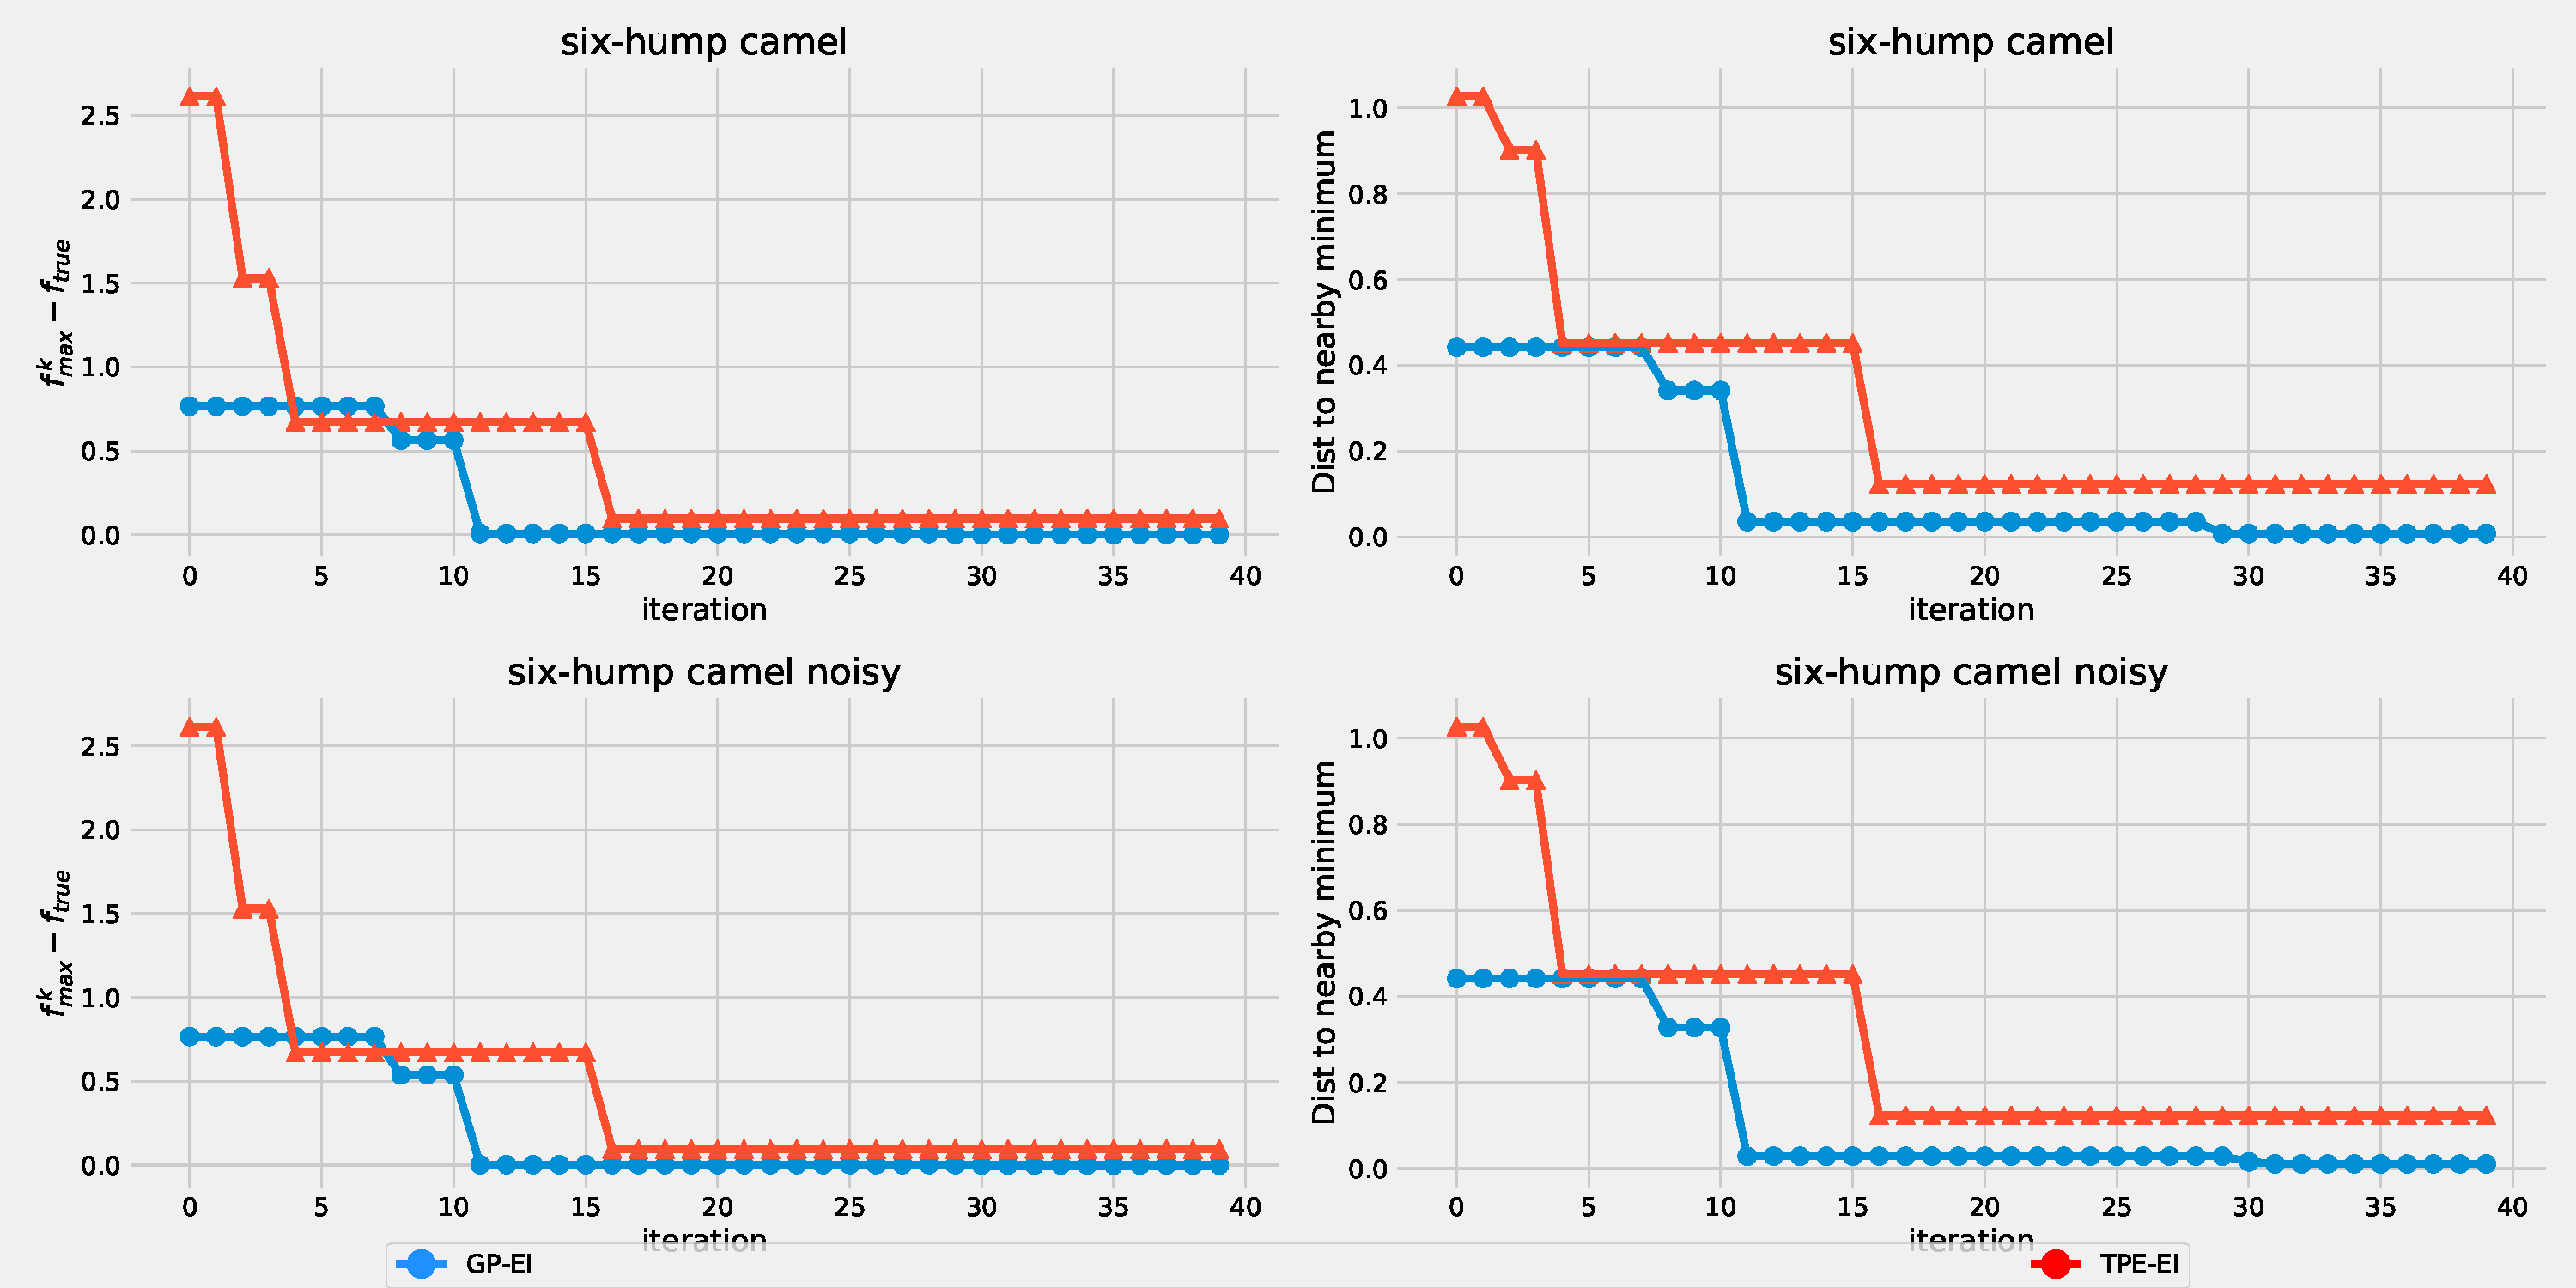
\includegraphics[scale=0.25,center]{../code/exp2/hump.pdf}
		\caption{\textbf{Эксперимент 2:} Six-Hump Camel Function}
		\label{fig:exp2_hump}
	\end{figure}
	
	\begin{figure}[!h]
		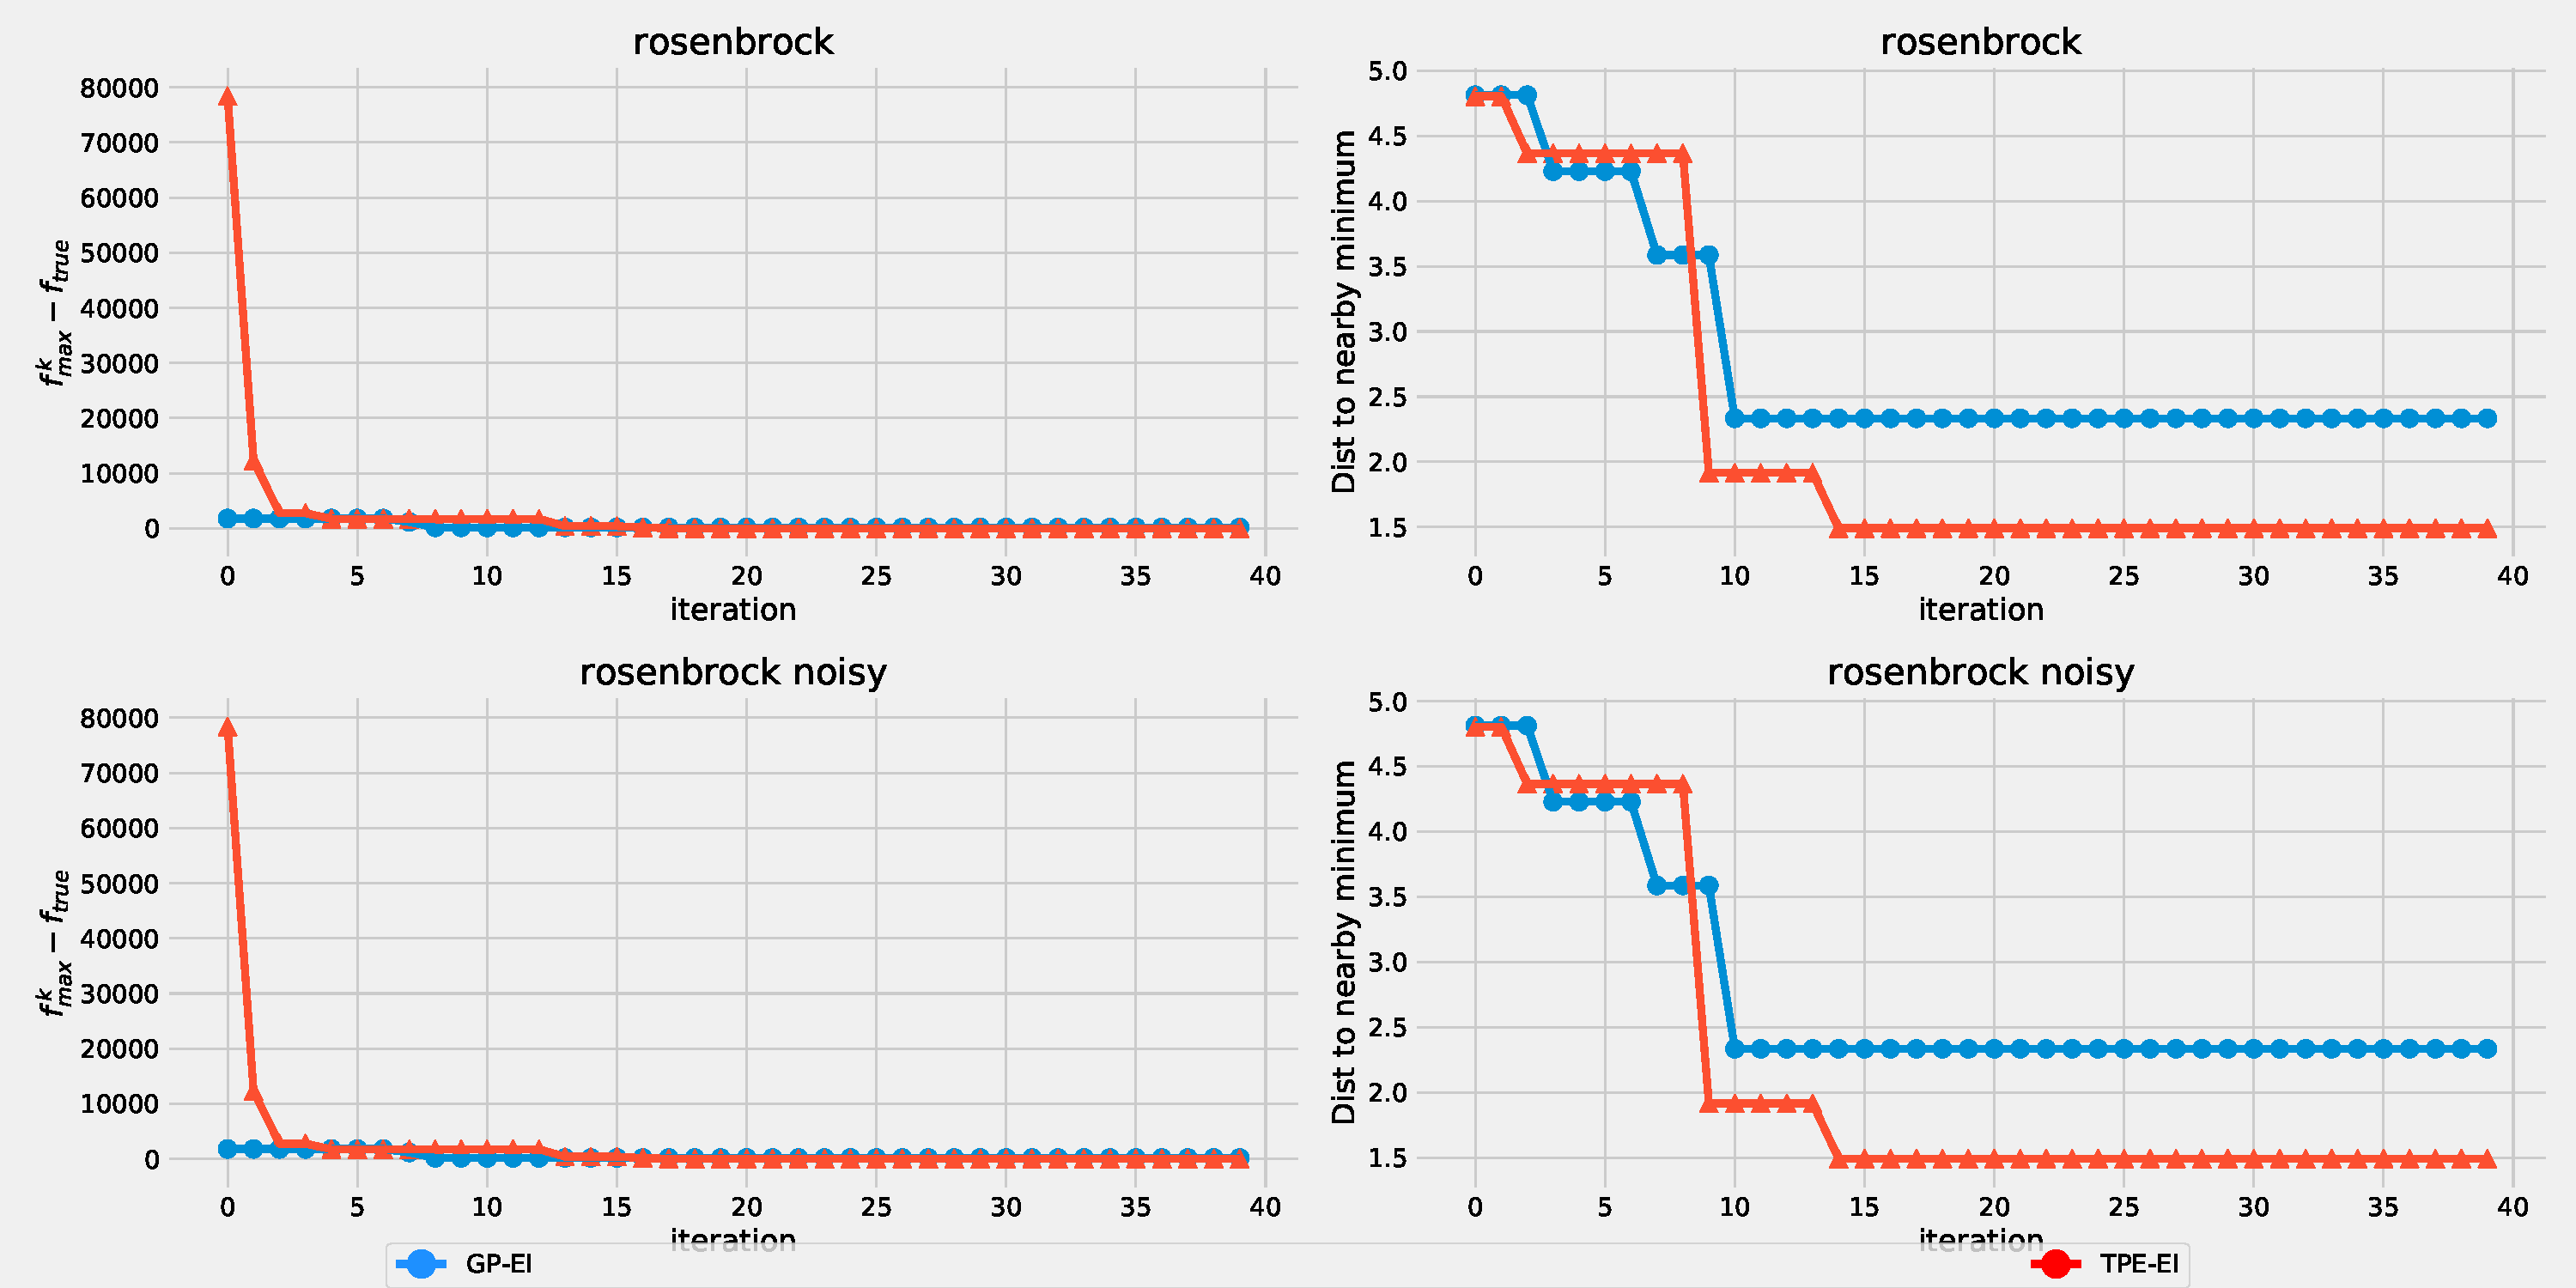
\includegraphics[scale=0.25,center]{../code/exp2/rosenbrock.pdf}
		\caption{\textbf{Эксперимент 2:} Rosenbrock Function}
		\label{fig:exp2_rosenbrock}
	\end{figure}
	
	\begin{figure}[!h]
		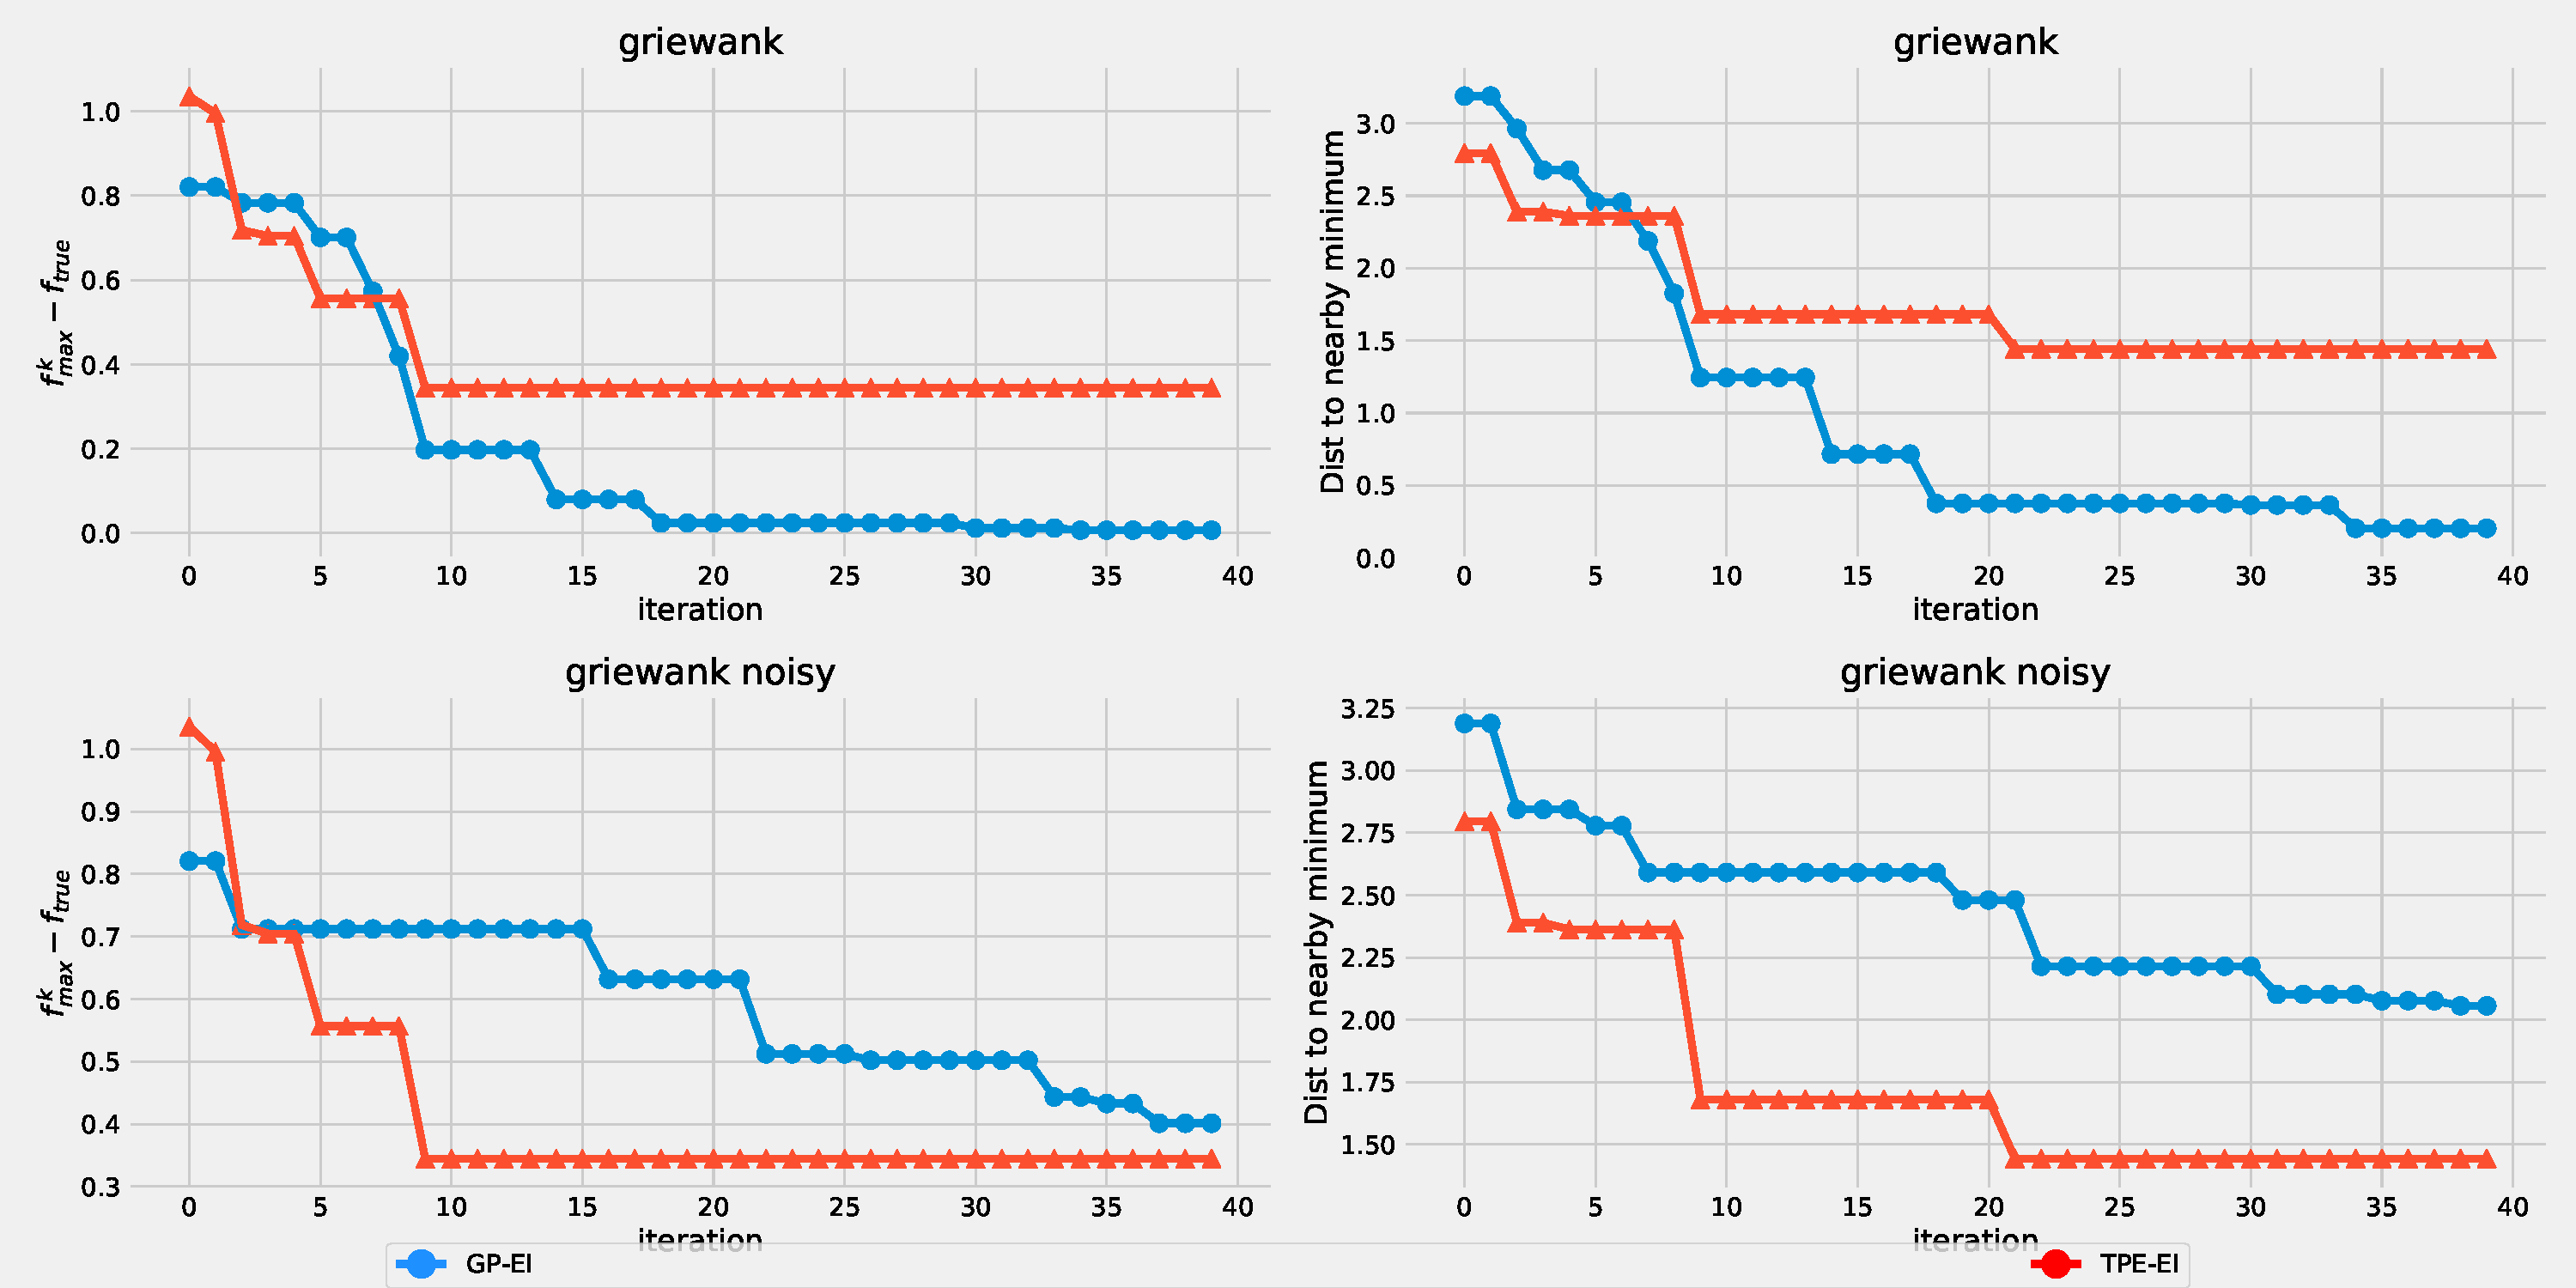
\includegraphics[scale=0.25,center]{../code/exp2/griewank.pdf}
		\caption{\textbf{Эксперимент 2:} Griewank Function}
		\label{fig:exp2_griewank}
	\end{figure}
	
	
	
	\newpage
	\subsection{Эксперимент 3}
	Предлагается исследовать влияние выбора ядра на качество и скорость сходимости.
	Рассматривался структура GP-EI. В качестве рассматриваемых ядер выбраны: настраиваемое и константные ядра Matérn 5/2 (MATERN5\_UPD, MATERN5\_FIX), Matérn 3/2 (MATERN3\_UPD, MATERN3\_FIX), Squared-Exponential (RBF\_UPD, RBF\_FIX). Результаты представленны на рисунках \ref{fig:exp3_branin}, \ref{fig:exp3_griewank}, \ref{fig:exp3_hump}, \ref{fig:exp3_rosenbrock}, \ref{fig:exp3_easom}, \ref{fig:exp3_colville}.
	
		Почти всегда методы с настраиваемыми параметрами работают лучше. Исключением является функция Easom, у которой один глобальный минимум, который максимизацей правдоподобия находится не будет, если не повезёт с выбором начальной точки, поскольку в области за кругом радиуса $\pi$ в точке $(\pi, \pi)$ она имеет значения близкие к 0. Поэтому модель будет настраиваться почти на константное значение около нуля. 
	\begin{figure}[!h]
		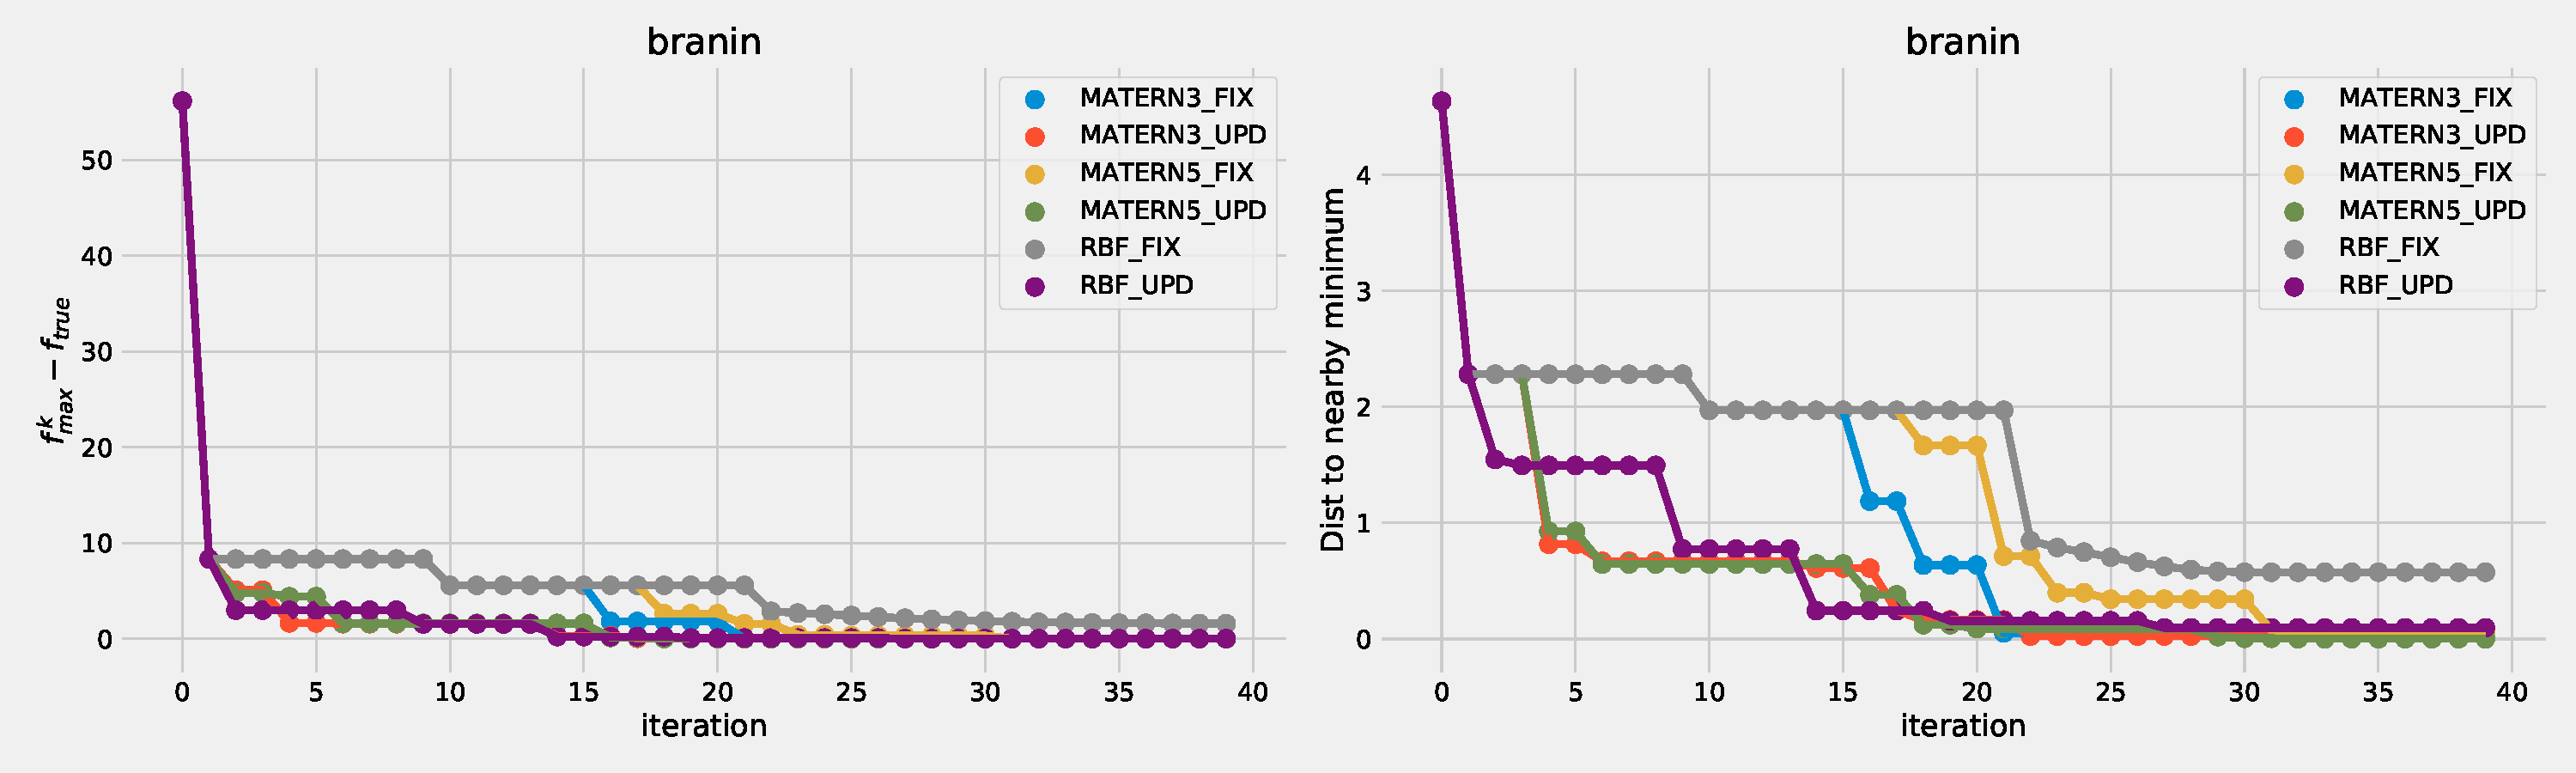
\includegraphics[scale=0.25,center]{../code/exp3/branin.pdf}
		\caption{\textbf{Эксперимент 3:} Branin Function}
		\label{fig:exp3_branin}
	\end{figure}
	
	\begin{figure}[!h]
		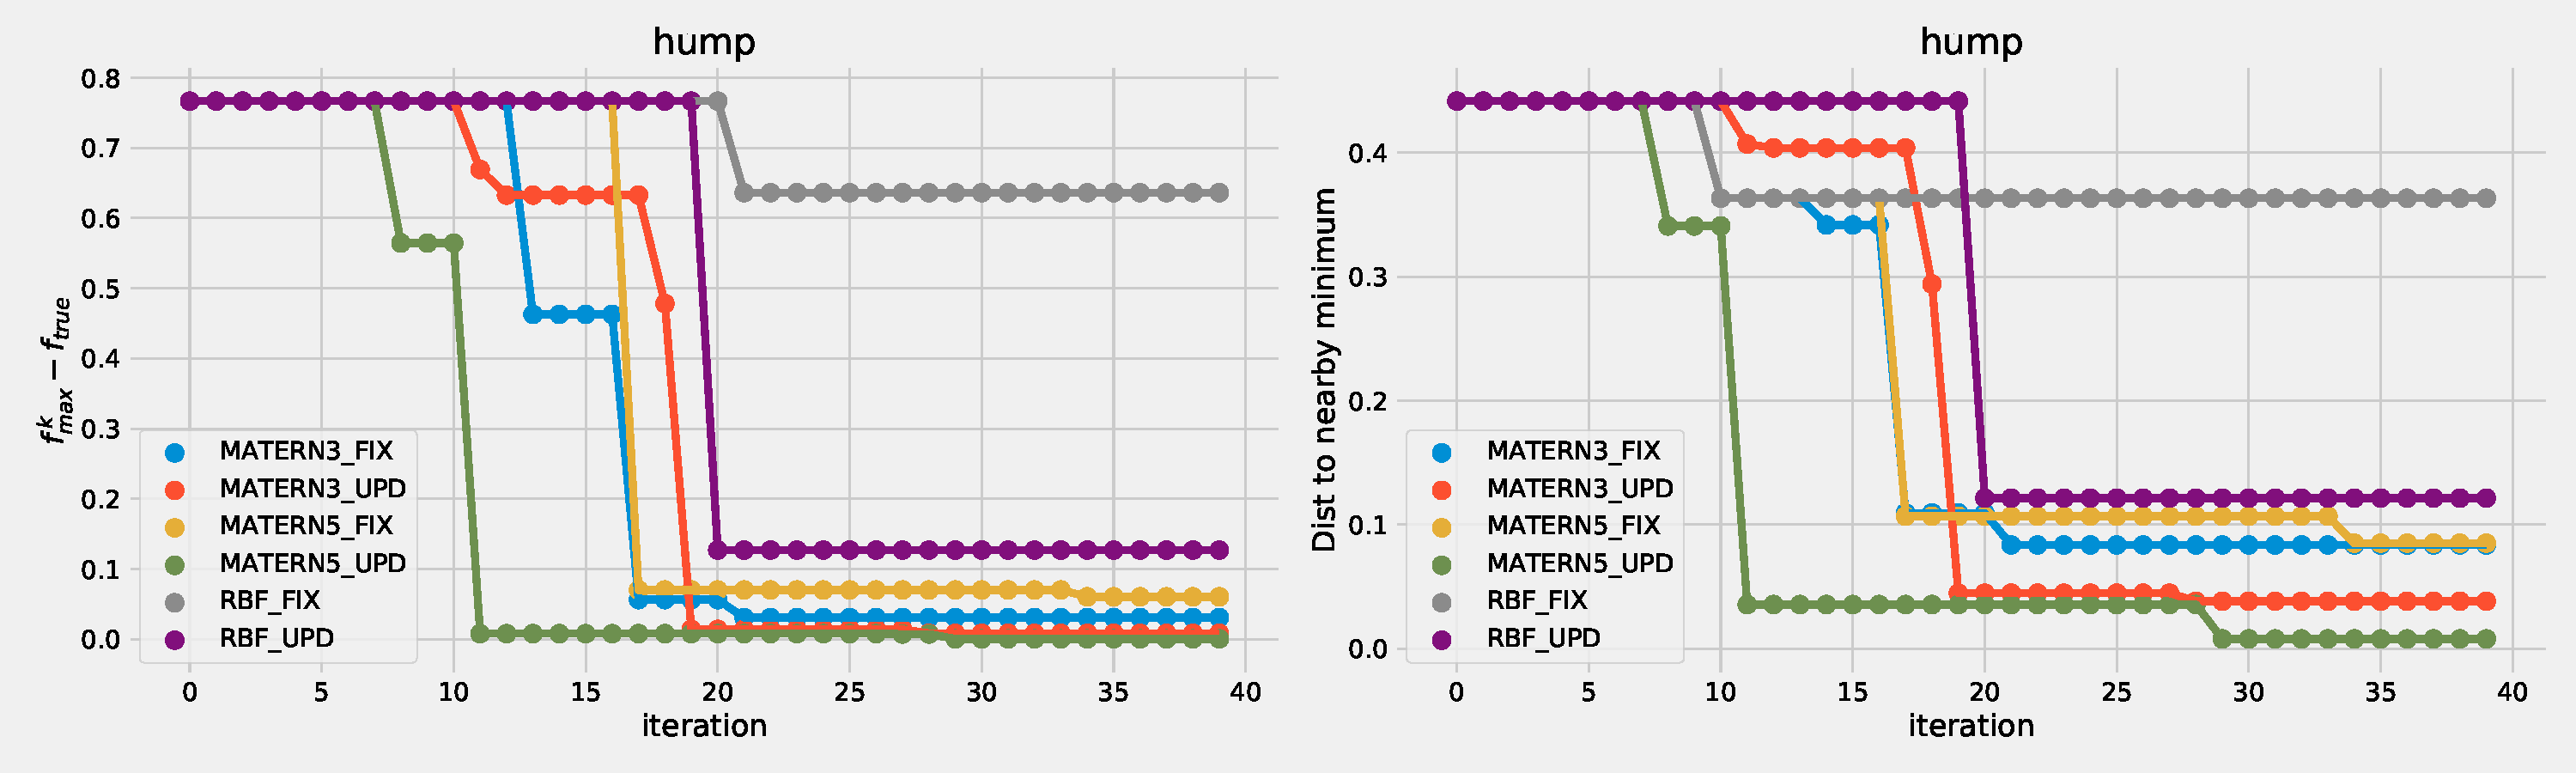
\includegraphics[scale=0.25,center]{../code/exp3/hump.pdf}
		\caption{\textbf{Эксперимент 3:} Six-Hump Camel Function}
		\label{fig:exp3_hump}
	\end{figure}
	
	\begin{figure}[!h]
		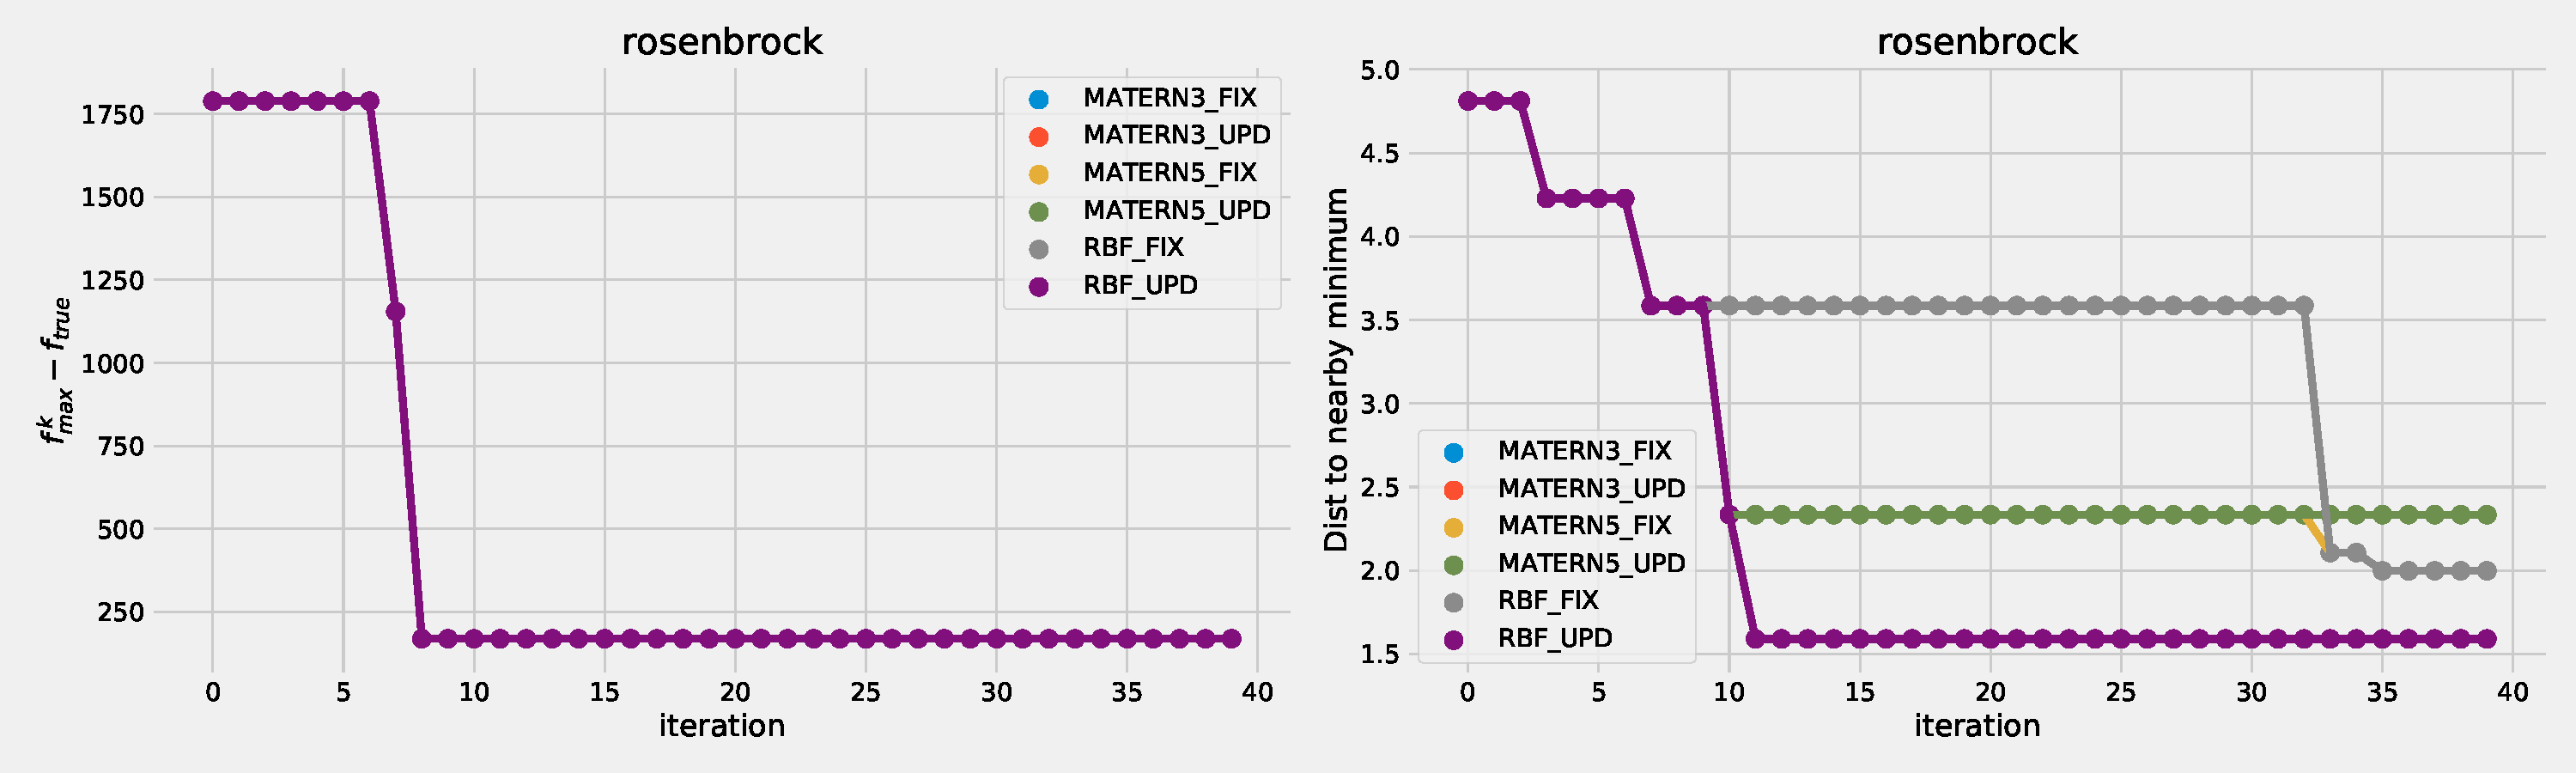
\includegraphics[scale=0.25,center]{../code/exp3/rosenbrock.pdf}
		\caption{\textbf{Эксперимент 3:} Rosenbrock Function}
		\label{fig:exp3_rosenbrock}
	\end{figure}
	
	\begin{figure}[!h]
		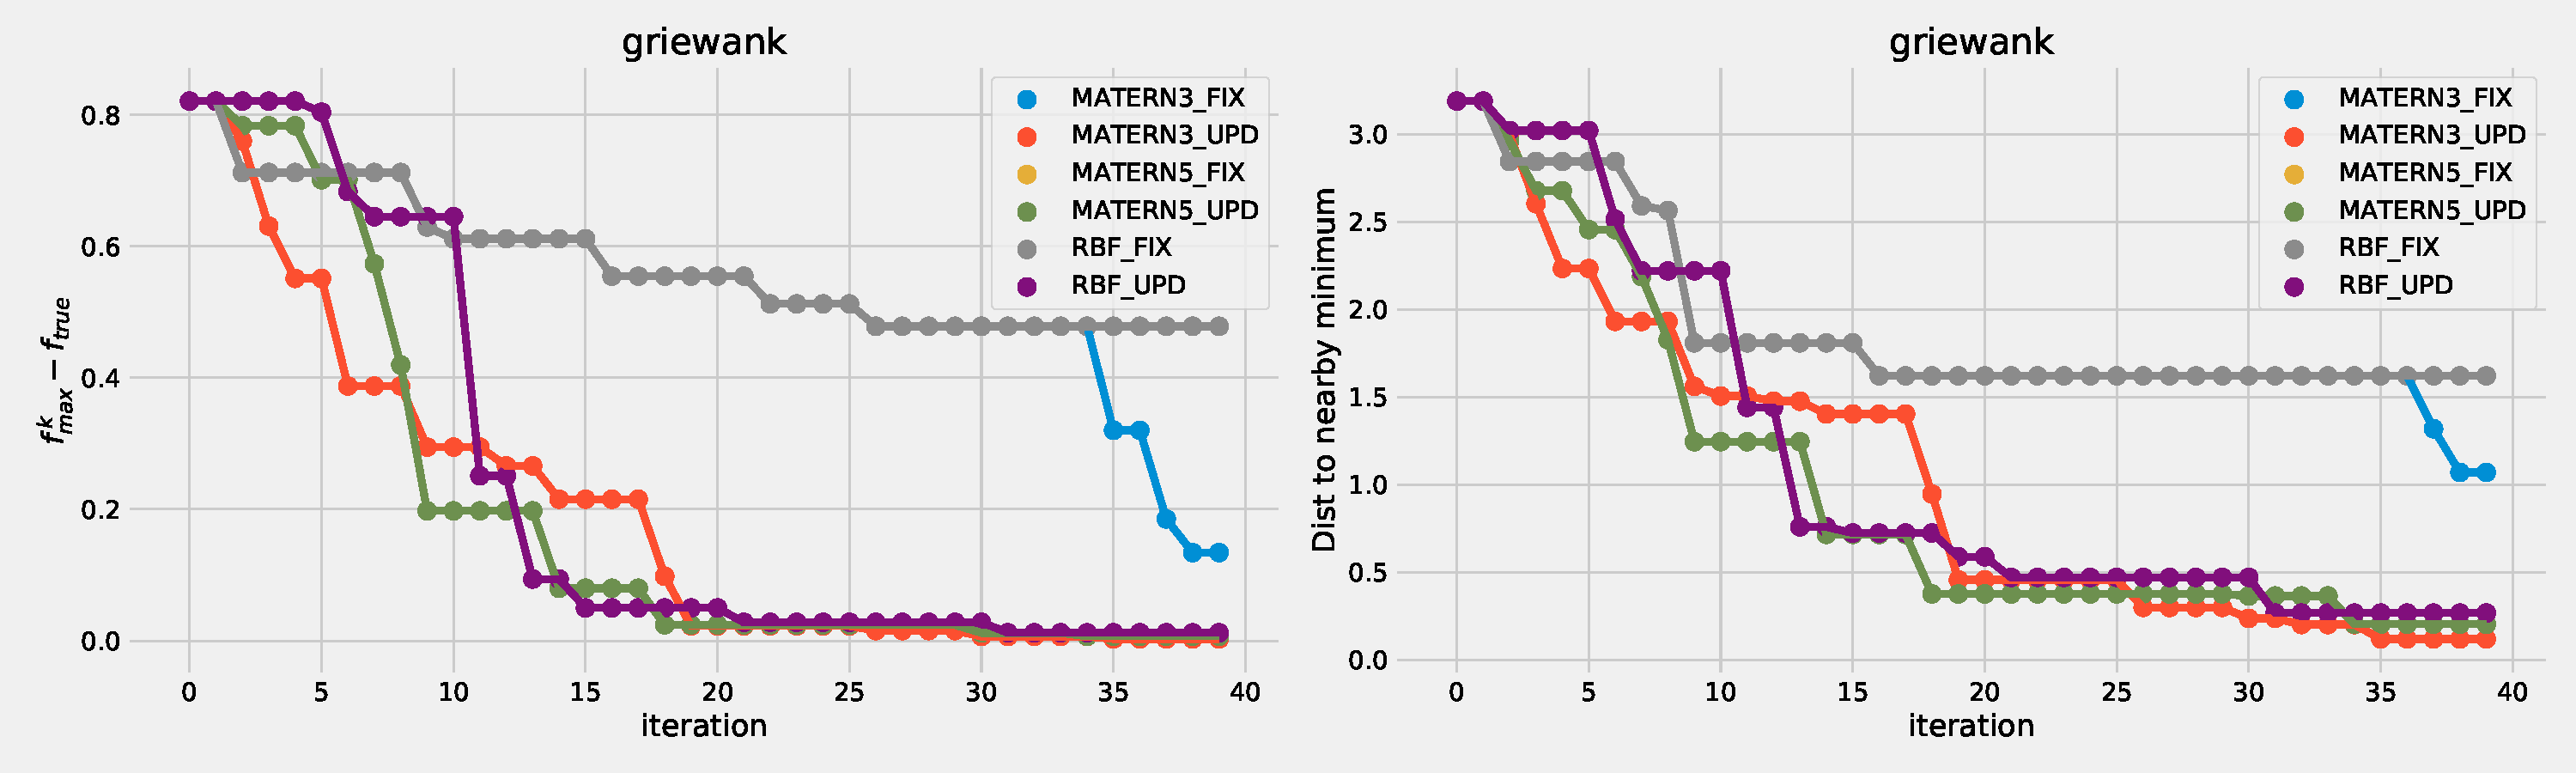
\includegraphics[scale=0.25,center]{../code/exp3/griewank.pdf}
		\caption{\textbf{Эксперимент 3:} Griewank Function}
		\label{fig:exp3_griewank}
	\end{figure}

	\begin{figure}[!h]
		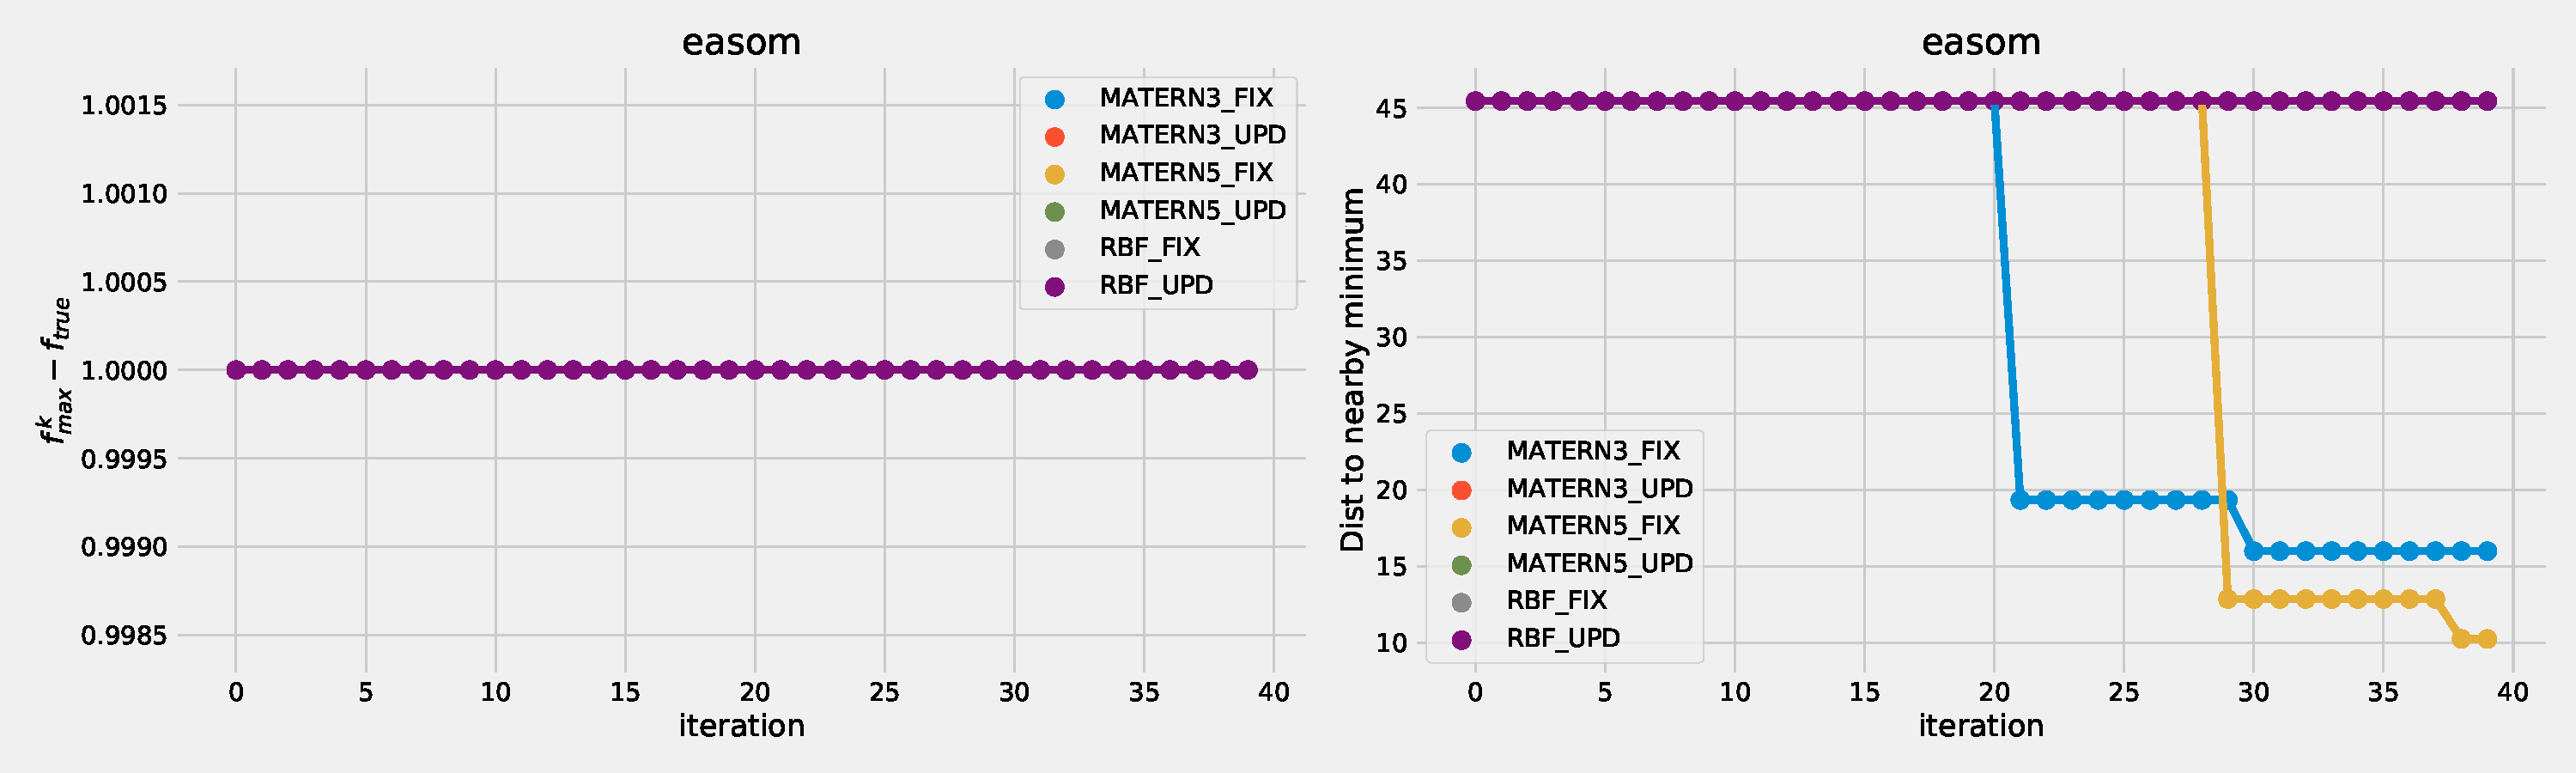
\includegraphics[scale=0.25,center]{../code/exp3/easom.pdf}
		\caption{\textbf{Эксперимент 3:} Easom Function}
		\label{fig:exp3_easom}
	\end{figure}
	
	\begin{figure}[!h]
		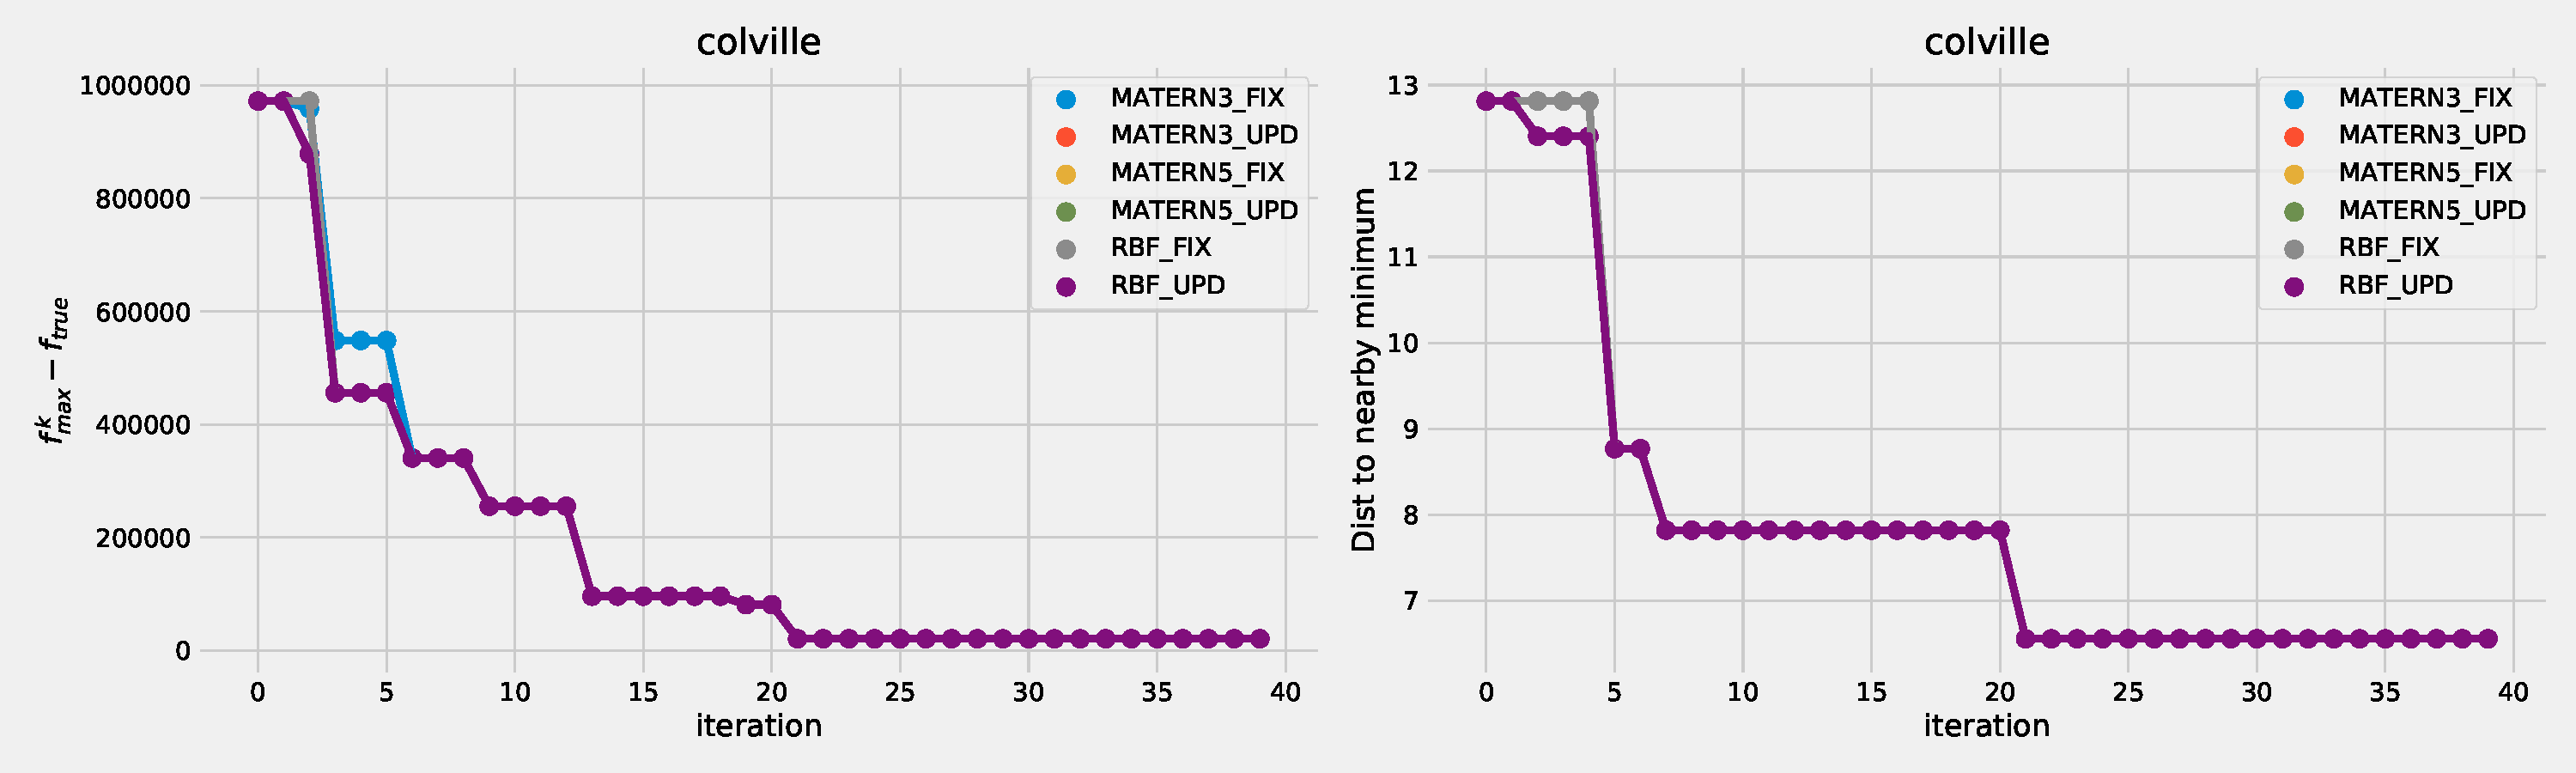
\includegraphics[scale=0.25,center]{../code/exp3/colville.pdf}
		\caption{\textbf{Эксперимент 3:} Colville Function}
		\label{fig:exp3_colville}
	\end{figure}
	

	
	\newpage
	
	\subsection{Эксперимент 4}
	Предлагается рассмотреть реальную задачу оптимизации гиперпараметров. В качестве обучаемой модели выбрана SVM. Рассматривается задача классификации изображений рукописных цифр из датасета MNIST. Каждое представляет из себя бинарную маску размера $28\times28$, на которых изображены 10 классов (цифры 0-9). Предлагается настраивать следующие параметры:
	\begin{itemize}
		\item Параметр C, отвечающий за штрафование ошибочных классификаций. Рассматривался отрезок $[1, 10^5]$;
		\item Параметр $\gamma$ радиально базисного ядра. Рассматривался отрезок $[10^{-5}, 10^{-1}]$.
	\end{itemize}
	Предлагается настраивать точность (accuracy) модели на тестовой выборке. В качестве методов оптимизации гиперпараметров рассматривались GP-PI, \mbox{GP-EI},\mbox{GP-UCB}, GP-PES, TPE-EI.
	
	Как и утверждалось ранее метод GP-UCB показывает сравнимо худшие результаты на старте, однако в конце за счёт маленького коэффициента $\beta_n$ настраивается лучше большинства методов (аналогия с learning-rate). GP-PES работает хорошо на старте, поскольку значение параметра C меняется в достаточно широком диапазоне. Методу TPE-EI повезло с выбором начального приближения, однако найти более лучшего претендента не удалось. Метод GP-EI хотя и сходился долго, но показал лучший результат.  
	
	\begin{figure}[h]
		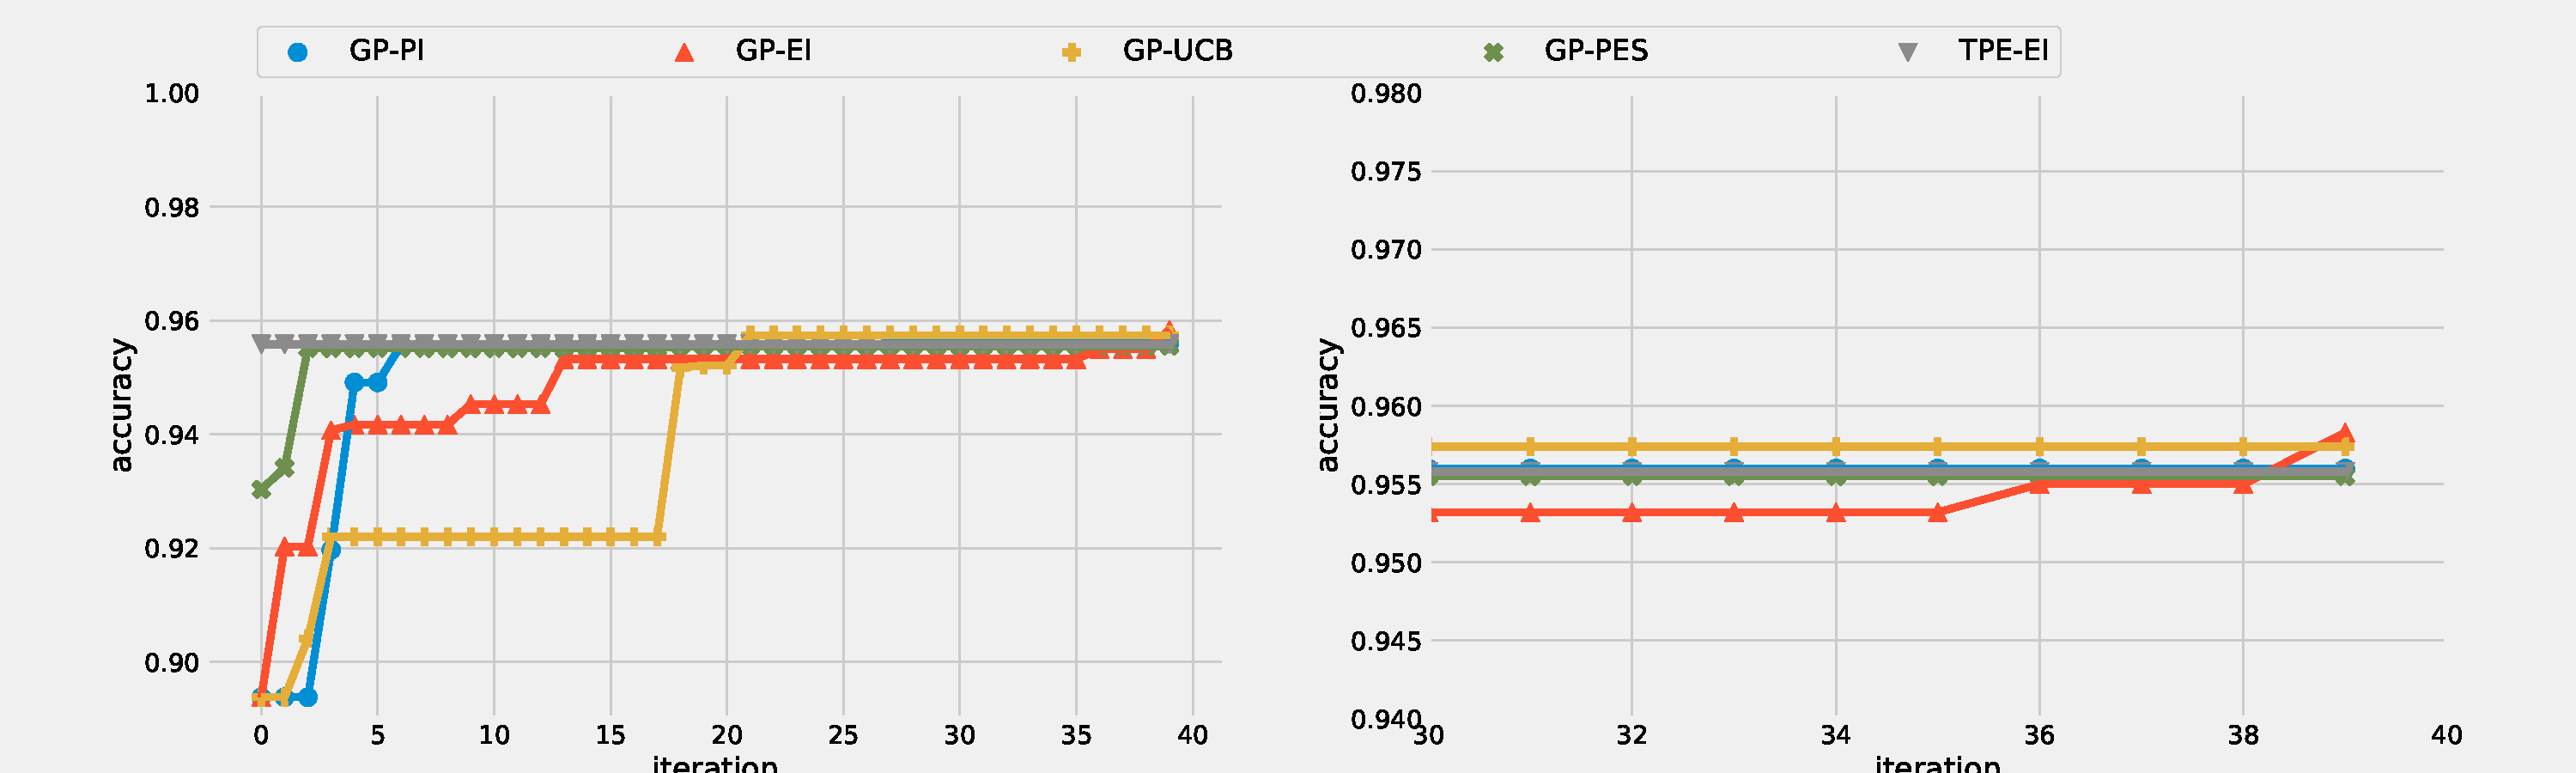
\includegraphics[scale=0.4,center]{../code/exp4/svm.pdf}
		\caption{\textbf{Эксперимент 4:} Классификация датасета MNIST с помощью SVM}
		\label{fig:exp4_svm}
	\end{figure}
	
	\subsection{Выводы из экспериментов}
	
	В результате экспериментов выявлено следующее:
	
	\begin{itemize}
		\item Выбор вспомогательной функции зависит от наличия шумовой компоненты в данных. При её наличии хорошим изначальным выбором будет Expected Improvement. В случае, если нужно донастроить модель лучше использовать UCB с маленьким шагом $\beta_n$;
		\item Выбор ядра должен основываться на виде данных, а сами ядра настраиваться в ходе обучения;
		\item Среди рассмотренных моделей выделить особой лучшей комбинации нельзя.
	\end{itemize}
	\newpage
\section{Заключение}

В ходе работы были изучены основные подходы используемые при оптимизации гиперпараметров. Были соответствующие вычислительные эксперименты. В ходе экспериментов установлено, что среди рассмотренных методов нельзя выделить лучшую комбинацию, выбор параметров моделей должен основываться на данных.

В качестве дальнейшей работы в рамках Байесовской оптимизации можно рассмотреть методы, комбинирующие представленные вспомогательные функции (Portfolios of Acquisition Functions). Также можно рассмотреть усложнённые варианты вероятностных моделей, например случайный процесс Стьюдента \cite{shah2014student}.

\newpage


\bibliographystyle{gost71s}
\bibliography{Literature}



\end{document}